\documentclass[11pt,letterpaper]{article}
\usepackage{graphicx}
\usepackage[hmargin=1in]{geometry}
\usepackage[T1]{fontenc}
\usepackage{txfonts}
\usepackage[font=footnotesize]{caption}
\usepackage{titling}
\usepackage{url}
\usepackage{pifont}
\renewcommand\labelitemi{\ding{109}}
\renewcommand\labelitemii{\ding{111}}
\graphicspath{{images/}}
\newcommand{\ident}[1]{{\tt #1}}
\newcommand{\display}{\mbox{MNI-Display}}
\newcommand{\menu}[1]{{\scriptsize \fbox{\bf #1}}}
\newcommand{\menutwo}[2]{{\scriptsize \fbox{\bf #1}/\fbox{\bf #2}}}
\newcommand{\menuthree}[3]{{\scriptsize \fbox{\bf #1}/\fbox{\bf #2}/\fbox{\bf #3}}}

\title{{\bf \display} - Software for Visualization and Segmentation of Surfaces and Volumes}
\author{Robert D. Vincent, Athena Buckthought, and David MacDonald}
\pretitle{
\begin{center}
\Large

\includegraphics[width=0.3\columnwidth]{neuro-logo.jpg}\\[\bigskipamount]
}
\posttitle{
\end{center}
}
\begin{document}

\maketitle

\setcounter{tocdepth}{2}
\tableofcontents

\newpage

\section{Introduction}

\display{} is a program originally written by David MacDonald as part of
this thesis research while a student at the McConnell Brain Imaging
Centre. The program was designed to display and manipulate three
dimensional objects, mainly human cortical surfaces and sulcal
curves. It has evolved to include visualization and segmentation of 3D
and 4D medical images. The user interface is a non-standard menu
oriented system based on keystrokes and mouse (or touchpad) operations.

\subsection{Visualization features}
\display{} supports a large number of visualization features.
\begin{itemize}
\item Support for overlaying multiple volumetric images irrespective of differences in their sample grid sizes.
\item Visualization of 3D surfaces, and the intersection of the 3D surface with the volumetric data.
\item The ability to display an oblique (non-orthogonal) plane through the volumetric data.
\item Flexible choices for mapping from voxel data to colours.
\end{itemize}

\subsection{Segmentation features}
\display{} allows a researcher to annotate structural features on either a surface or a volumetric dataset.
\begin{itemize}
\item Support for per-voxel labeling of volumetric data.
\item Arbitrary mapping from label values to colours.
\item Powerful fill, dilation, and erosion operations.
\end{itemize}

\subsection{Coordinate system}

Most medical image files can be thought of as having two different,
but equally important coordinate systems. The first system is called
{\em voxel} coordinates in this document. By voxel coordinates we mean
the position of a particular voxel in the absolute reference frame of
the sampled data. Since medical images are generally sampled at
discrete points in time and space, voxel coordinates are naturally
also discrete, and numbered from zero to $N_i-1$ where $N_i$ is the
number of sample points along voxel dimension $i$.

In contrast, {\em world} coordinates refer to the actual position of
the patient with respect to the image. In this document, we define
that the world X-axis always increases from patient left to patient
right, the Y-axis increase from patient posterior to anterior, and the
Z-axis increases from patient inferior to superior.

\begin{figure}
\centering
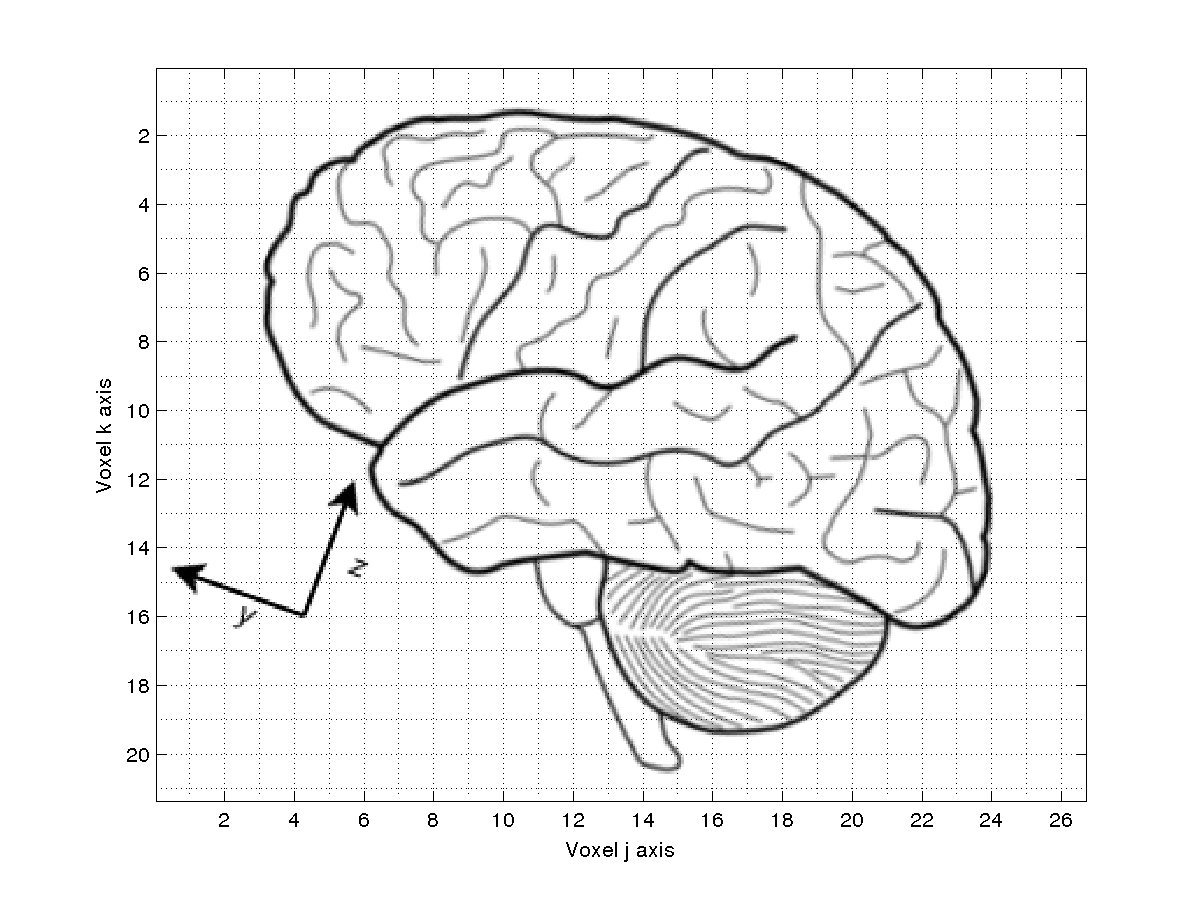
\includegraphics[width=0.75\linewidth]{coordinates.png}
\caption[Voxel vs. world coordinates]{Voxel vs. world coordinates. Each square represents a single sample in the voxel space of the image. The voxel origin (0,0) would be in the upper left corner of the image. The world Y and Z directions
are rotated 20 degrees relative to the voxel coordinates. The origin of the world coordinate system would be defined with respect to some anatomical landmark.}
\label{figCoord}
\end{figure}
Most medical image formats define a transformation from voxel
coordinates to world coordinates. \display{} always defines a current
{\em cursor} position within the space, and keeps of this position
with respect to both coordinate systems.

When displaying a single volume, \display{} will show the volume
oriented in its original voxel coordinate frame, attempting to orient
the image such that the voxel axis closest to the world X axis, for
example, will be used as the X axis in the image.

When displaying multiple volumes, \display{} will re-orient subsequently
loaded volumes so that their world coordinates are consistent with
those of the first loaded volume.

\section{What's new in Version 2.0}

A number of major features have been added in \display{} 2.0. Many of
the features are cosmetic or user interface improvements, others
involve core functionality.

\subsection{Core functions}
\begin{itemize}
\item The intersection between a 3D surface and the loaded volume is automatically displayed in the slice window.
\item Dynamic scans (e.g. DTI, fMRI, and PET) can now be loaded in \display{}.
\item Input support for FreeSurfer (.MGZ/.MGH) and NIfTI-1 (.NII) volumes.
\item The previous 20 painting operations can be undone.
\item A user can now load per-vertex data, such as cortical thickness measurements, for visualization on 3D surfaces.
\end{itemize}

\subsection{User interface}
\begin{itemize}
\item Users can now save and restore their preferred window positions and sizes.
\item Dynamic help text is displayed for each menu command.
\item Better integration with modern mice and trackpads.
\item Addition of new information in the 3D View and Slice View windows.
\item New mouse and key bindings to speed access to important commands.
\item User interaction can now use a graphical interface rather than the
terminal window.
\end{itemize}

The new version also includes many bug fixes and performance inprovements.

\section{Installing and Running \display{}}

\display{} runs on most POSIX-compliant operating systems, including Linux
and Mac OS X. You may find that \display{} is already installed on your workstation.

\subsection{Installing \display{}}
If you do not already have \display{} installed, you can install it as
part of Minc Tools (version 1.0.01 is recommended), following the
instructions at:
\url{http://www.bic.mni.mcgill.ca/ServicesSoftware/ServicesSoftwareMincToolKit}.

Alternatively, the source code for MNI-Display is available on Github:
\url{https://github.com/BIC-MNI/Display}.

Once you have installed the program, you must also source the
environment before you can run it.  That is, if you installed it to
/opt/minc, then you must type in the terminal window:
\begin{verbatim}
  source /opt/minc/minc-toolkit-config.sh # (for bash)
\end{verbatim}
or
\begin{verbatim}
  source /opt/minc/minc-toolkit-config.csh # (for tcsh)
\end{verbatim}

Change these directories if it you installed the toolkit to a
different location. Then you should be ready to run the program.

More information about MNI-Display is also available at:
\url{http://www.bic.mni.mcgill.ca/software/Display/Display.html}
and
\url{http://www.bic.mni.mcgill.ca/~david/}.

\subsection{Running \display{}}

To run \display{}, type the following in a terminal window:

\begin{verbatim}
    Display  [file1]  [file2]  ... [fileN]
\end{verbatim}

where each file is one of:

\vspace{.5cm}

\begin{itemize}
\item A volumetric image, containing an MRI, PET, or other 3 or 4 dimensional volume, with a filename extension \ident{.mnc}, \ident{.nii}, or \ident{.mgh}.

\item A 3D object file containing 3D surfaces, lines, or other objects, and
with the filename extension \ident{.obj}.

\item A tag point file containing a list of 3D points, such as those chosen from a volume, with the filename extension \ident{.tag}.

\item A colour map file that contains a list of label values followed by colour 
codes, with the file extension \ident{.map}.
\end{itemize}

Note that the above files may be compressed.  If the file ends in
\ident{.gz}, then it is compressed and the full name of the file, including the
\ident{.gz}, must be specified to \display{}.

Note that you can load more than one of either the volumetric images or
the 3D object files. If you do load multiple files of the same type,
they will be displayed in the appropriate window
simultanously. \display{} will attempt to overlay the two images, as
long as they are in approximately the same location relative to the
world coordinate space.

Command line options to \display{} are keywords introduced with a dash
('-') character, often with one or more additional arguments. Supported
options include:

\begin{itemize}
\item \ident{-help} : Print basic usage information and exit.
\item \ident{-version} : Print program and library version information and exit.
\item \ident{-label} $filename$ : Load volume labels from the given file in \ident{.mnc} or \ident{.tag} format.
\item \ident{-skiperror} : Ignore errors encountered when loading files from the command line.
\item \ident{-ratio} $V_1$,$V_2$ : Display the value of volume number $V_1$
  divided by value of volume number $V_2$ as part of the slice window status. You must load at least two
  volumes for this option to have any effect.
\item \ident{-global} $name$ $value$ : Set the configuration variable of the given name to the specified value. \display{} supports an extremely large number of configuration options, many of these are described in Section \ref{secGlobals}.
\item {\bf Initial range options:} These options request \display{} to
  use different approaches to setting the initial range of the colour
  mapping used to convert voxel values into colours. They each set two
  values, $M_{min}$ and $M_{max}$, that define this range. Voxel values
  less than $M_{min}$ are assigned the ``under'' colour, and voxels
  greater than $M_{max}$ are assigned the ``over'' colour.
\begin{itemize}
\item \ident{-range} $A_{min}$ $A_{max}$ : Set the initial range used to
  map volume data to colours to the {\em absolute} values specified. The
  value $A_{min}$ should be less than $A_{max}$.
\item \ident{-rel\_range} $R_{min}$ $R_{max}$ : Set the initial range used to
  map volume data to colours to the {\em relative} values specified as a
  fraction of the total data range, $M_{min} = V_{min} + R_{min}
  (V_{max} - V_{min})$ where $(V_{min},V_{max})$ is the real range of
  the voxel data. For example, if $R_{min}=0.2$, $V_{min}=-1.0$, and 
  $V_{max}=+1.0$, then $M_{min}=-0.6$.
\item \ident{-hist\_range} $P_{min}$ $P_{max}$ : Set the initial range used to
  map volume data to colours to the percentile values specified. For
  example, a $P_{min}$ value of 0.2 attempts to set $M_{min}$ such that
  20\% of all voxels will have values below the colour coding range.
\end{itemize}
\item {\bf Volume colour coding options}:
\begin{itemize}
\item \ident{-gray} : Use grayscale colour map for subsequently loaded volumes.
\item \ident{-hot} : Use hot colour map for subsequently loaded volumes.
\item \ident{-spectral} : Use spectral colour map for subsequently loaded volumes.
\item \ident{-red} : Use red colour map for subsequently loaded volumes.
\item \ident{-blue} : Use blue colour map for subsequently loaded volumes.
\item \ident{-green} : Use green colour map for subsequently loaded
  volumes.
\end{itemize}
\end{itemize}

The colour mapping options normally apply to the volumes specified after
the option, and these options can be repeated to set different values
for subsequently loaded volumes. For example:

\begin{verbatim}
Display -gray -rel_range 0.1 0.9 t1.mnc -spectral -range 0 1000 rs.mnc
\end{verbatim}
would load the first volume with the gray colour map and
the colour coding range set at 10\% and 90\% of the real voxel
range. The second volume would be loaded with the spectral colour map
and absolute colour coding range set to 0, 1000.

\section{\display{} Windows}
When \display{} starts, it normally creates up to four different
windows. Each window has a specialized purpose.

\begin{itemize}
\item The 3D view window displays the 3D objects, such as surfaces, lines,
and markers. If no 3D objects are loaded, it may not be displayed.
\item The slice window displays up to 4 views of slices through one or more 
volumes. If no volumes are loaded, it may not be displayed.
\item The menu window shows the current menu command options.
\item The object window shows a list of the currently loaded 3D objects.
\end{itemize}

\subsection{Menu Window}

\begin{figure}
\centering
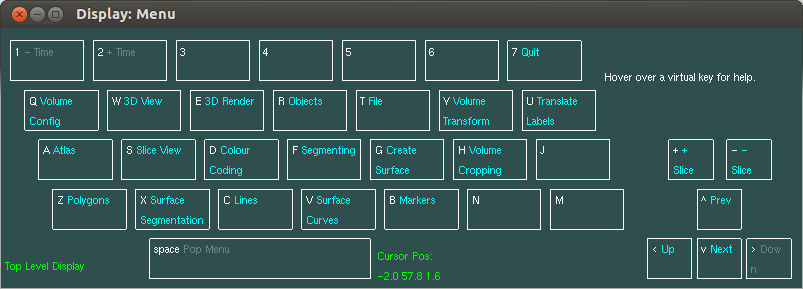
\includegraphics[width=0.9\textwidth]{display-top-menu.png}
\caption{The menu window}
\label{winMenu}
\end{figure}

The menu window (Figure \ref{winMenu}) contains the representation of
the partial keyboard, the name of the currently selected menu in the
lower left corner.

The current cursor position (in {\em world} coordinates) is displayed
in the lower central part of the menu window. The cursor position will
include the X, Y, Z, and time coordinates as appropriate.

As you move the mouse cursor over a key image displayed on the menu
window, a brief text message describing the function of that key will
be displayed in the upper right corner of the menu window.

Any right mouse click on a key image will invoke the function
associated with that key, if the key image is not ``grayed out''. The
function associated with a key may either be a submenu or an actual
command.

A middle mouse click in the menu window will return the menu back up a
level, similar to the operation of the space bar.

This window always has the title ``Display: Menu''.

\subsection{Object list window}

\begin{figure}
\centering
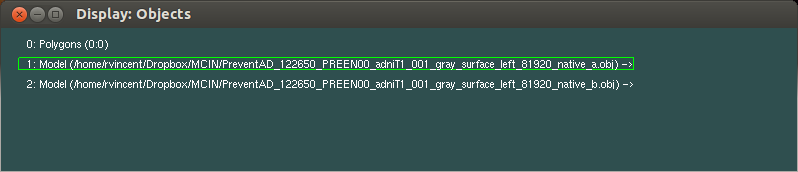
\includegraphics[width=0.9\linewidth]{display-obj-list.png}
\caption{The object list window}
\label{winObjList}
\end{figure}

All 3D objects loaded and created in \display{},
(with the exception of volumes) are listed in the object hierarchy. The
arrow keys are used to move around in this hierarchy and to select the
current object. Also, clicking on an object in the 3D view window or on the
name of the object in the object list hierarchy with the left mouse button
will make it the current selection.

The 3D objects used by \display{} may be one of several types. They may
be {\em markers} that record a single 3D position. They may be {\em
 polygons} that represent a complex surface using a series of points
or vertices to create a triangular mesh. They may be {\em lines} that
represent a simple curve or shape. Finally, {\em model} objects act as containers for any number of other objects, including other models.

This window always has the title ``Display: Objects''.

\subsection{3D View Window}

\begin{figure}
\centering
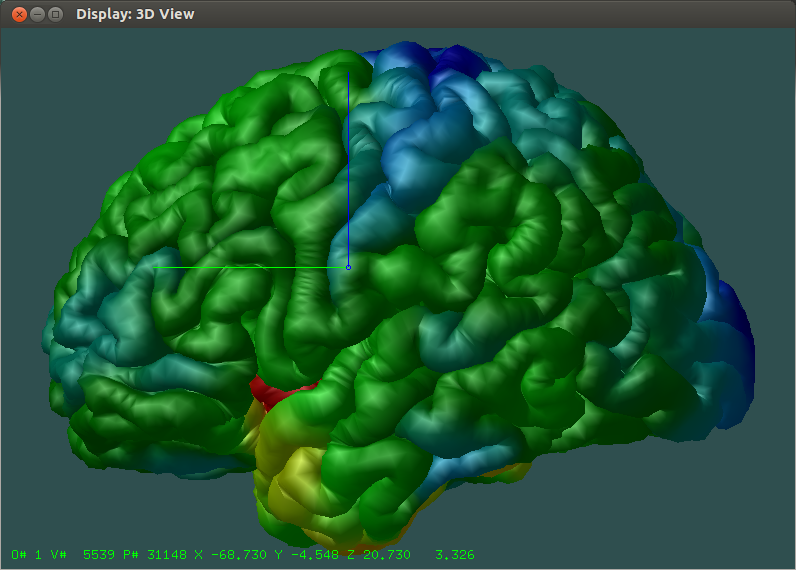
\includegraphics[width=0.7\linewidth]{display-3d-view.png}
\caption{The 3D View window}
\label{win3Dview}
\end{figure}

The 3D View window shows three-dimensional objects such as surfaces and
lines, with lighting and camera control. A representation of the cursor is 
also generally visible as a set of three coloured lines, where the X-axis is red, the Y-axis is green, and the Z-axis is blue.

A user can also select per-vertex data, such as cortical thickness
measurements, which may be used to ``colourize'' the 3D image.

In the 3D window, the following mouse operations are available:

\begin{itemize}
\item Left Button: Sets the current cursor position, and makes the 
object under the mouse the current object in the Object list window.
\item Middle Button: If the mouse is not near the cursor, rotates the 3D
objects around the cursor. If the mouse is close to the cursor, translates
the cursor along the axes.
\item Right button: translates the position of the 3D objects within the
window.
\item Scroll wheel: zooms the 3D objects.
\item Shift-Left Button: While holding down the \ident{shift} key, the
 left mouse button translates the position of the 3D objects within
 the window.
\item Control-Scroll wheel: Changes the opacity of the selected volume.
\end{itemize}

The 3D window also contains a ``status line'' that gives information about
the object relative to either the cursor or the mouse pointer. The fields
in this status line are enumerated in Table \ref{tab3DFields}.

If the mouse pointer is over a 3D object, the status line displays the
object number (relative to the list in the Object list window), the
vertex number, the polygon number, and the vertex coordinates closest
to the mouse pointer. If the mouse pointer is {\em not} over the 3D
object, this information is displayed relative to the current cursor
position.

\begin{table}
\centering
\caption{Fields displayed in the lower-left corner of the slice view window.}
\begin{tabular}{lp{0.8\linewidth}}
Label & Description \\
\hline
\ident{O\#} & The index (number) of the nearest object. \\
\ident{V\#} & The index of the nearest vertex. \\
\ident{P\#} & The index of the nearest polygonal face. \\
\ident{X Y Z} & The coordinates of the nearest vertex. \\
\ident{D} & The value of the per-vertex data for that vertex, if loaded. \\
\hline
\end{tabular}
\label{tab3DFields}
\end{table}

If per-vertex surface data is also loaded, that value associated with
the current vertex will be displayed as well. If no value is associated
with the vertex, the value field will display as a series of eight 
dash characters.

\subsection{Slice Window}

\begin{figure}
\centering
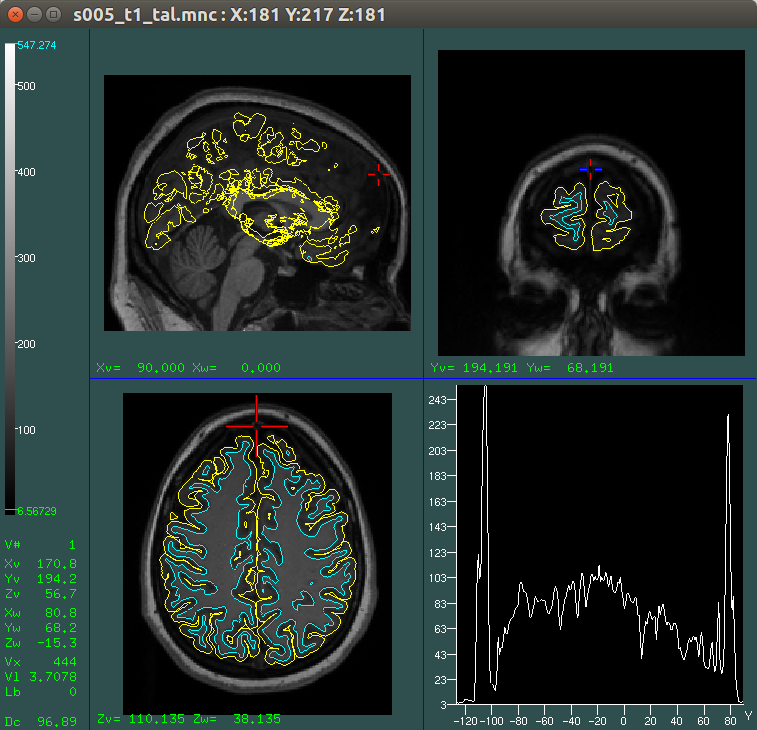
\includegraphics[width=0.8\linewidth]{display-slice.png}
\caption{Slice window showing the three orthogonal planes. Normally,
 the upper left quadrant will display the sagittal plane, the upper
 right will display the coronal plane, and the lower left will
 display the transverse plane. The lower right quadrant will display
 the optional oblique plane if enabled (Section \ref{secOblique}).}
\label{winSlice}
\end{figure}

The slice window displays slices of the loaded volumes, with various
options for mapping the voxel intensities into colours. Normally the
three orthogonal planes of a volumetric image will be displayed: The
sagittal in the upper left, the coronal in the upper right, and the
transverse in the lower left. The lower right quadrant is generally
used to display an optional oblique slice through an arbitrary plane.

In each of the three orthogonal quadrants, the width and height of the
field-of-view is displayed in world units near the top of the
quadrant, and the current slice position in voxel coordinates is
displayed near the bottom of the quadrant.

The far left side of the window contains the colour bar that is used
to show and control the current mapping of voxel intensities to
colours. 

In the lower left corner there is also a numeric display that shows a
number of useful value about the voxel under the mouse pointer, as
detailed in Table \ref{tabSliceFields}.
\begin{table}
\centering
\caption{Fields displayed in the lower-left corner of the slice view window.}
\begin{tabular}{lp{0.8\linewidth}}
Label & Description \\
\hline
\ident{V\#} & The index (number) of the current volume. \\
\ident{Xv Yv Zv} & The location of the mouse pointer in voxel coordinates. \\
\ident{Xw Yw Zw} & The location of the mouse pointer in world coordinates. \\
\ident{Vx} & The raw voxel intensity. \\
\ident{Vl} & The scaled voxel intensity. \\
\ident{Lb} & The voxel label value. \\
\ident{n/m} & The ratio between volume $n$ and volume $m$, if enabled. \\
\ident{Dc} & The distance from the cursor to the mouse pointer in world units. This field can also show the distance from a marker to the mouse pointer, in which case the label will show the number of the marker rather than the letter 'c'. \\
\hline
\end{tabular}
\label{tabSliceFields}
\end{table}

For each loaded volume, the slice window automatically associates
another volume of the same size as the loaded volume, which is
referred to as the {\bf label volume}. The label volume may be
explicitly loaded by the user, but if no such volume is loaded, an
empty label volume will be created. Each voxel of the label volume
typically is a small integer value (in the range 0-255), where a value
of zero means no label has been selected for this voxel. Each label
value is also associated with a colour. This colour mapping is
initialized to a set of internal values automatically, but you can
load a specific colour mapping using either the command line or menu
system.

In other words, every loaded volume has one ``voxel'' colour map that
is used for translating the values of the original volumetric dataset
into a set of colors, and there is a second ``label'' colour map used
to translate each user-assigned label value into a colour.

The slice window will also display a ``trace'' of any registered
surface that is displayed in the 3D View window. These traces
represent the intersection between the surface and the plane in the
current slice view(s).

In the slice window, the following mouse operations are available:

\begin{itemize}
\item Left Button: Sets the current cursor position.
\item Middle Button: Moving the mouse up or down while holding down
  the middle button changes the current volume slice position.
\item Right Button: Paints a region of the current volume slice with the
current brush label and size.
\item Shift-Left Button: While holding down the \ident{shift} key, the
  left mouse button translates the position of the slice within the
  viewport.
\item Shift-Middle Button: While holding down the \ident{shift} key,
  holding down the middle button and moving the mouse pointer up or down
  changes the magnification of the current slice.
\item Shift-Right Button: While holding down the \ident{shift} key,
  holding down the right button erases regions of the labels.
\item Scroll: The scroll wheel changes the zoom level of the current slice.
\end{itemize}

The upper and lower limits of the colour bar for the current volume
can be moved individually by pressing the left mouse button on the bar
near the desired limit. Pressing the middle button on the colour bar
will allow both limits to be moved simultaneously.

The relative sizes of the four slice views can be adjusted by clicking
and dragging with the right button down while the mouse cursor is
close to the intersection of the dividing lines between the slices.

\section{Menu and Interaction System}

The menu window (Figure \ref{winMenu}) represents the
layout of the left side of the keyboard.  A menu entry is selected by
hitting the corresponding key in any of the 4 \display{} windows, or
by pointing to the entry in the menu window with the mouse and
clicking the left button. The space bar will pop back one level in the
menu (as will the middle mouse button, when the mouse is over the menu
window). If the display of a menu entry is ``grayed out'' (in a
low-contrast colour), then this signals that the command is not valid
in the current context and cannot be selected.

In the remainder of this document the following convention will be
used to refer to menu selection: \menutwo{3D View}{Reset View} means
select the \ident{3D View} menu, then select the \ident{Reset View}
button from within the \ident{3D View} menu.

Whenever text must be typed, such as in prompts for filenames, size
and width parameters, etc., \display{} will attempt to display a
subwindow or ``dialog box'' that prompts for the information
requested. Each of these dialog boxes contains an \ident{OK} and
\ident{Cancel} button - selecting the \ident{Cancel} button should
always stop the requested operation without changing anything.

Some menu items cannot be selected by the mouse because the mouse must
be used to point to the object of the action, usually one of the 4
volume slices in the slice window.  In these cases, the mouse must be
positioned over the relevant slice in the slice window and the
keyboard character corresponding to the menu entry pressed.

Whenever the user is prompted to type in a colour, either the name of
a colour, such as \ident{red}, \ident{yellow}, or \ident{pink}, or a
numerical list of red-green-blue values, such as \mbox{\ident{0.3 0.7 0.7}}
(or \mbox{\ident{0.3 0.7 0.7 0.5}} for a semitransparent colour) may
be entered.

\section{Complete Menu Reference}

The following is a complete listing of every menu selection, with a
short description of each function. Since this program is also partly
a research tool, a few selections are not relevant to most users, and
will simply be described as not for general use. Figure \ref{winMenu}
shows the top level menu that is presented upon program start up, or
after popping the menu to the top level.

\subsection{Current Object}

The 3D graphics objects, as displayed in the 3D window, are also
presented in a hierarchical form in the object list window, as a tree
structure with each element of the tree being the name of a 3D
graphics object. There are 4 keys that can be used to navigate through
the list, where the currently selected object is always displayed with
a surrounding box:

\begin{description}
\item[\menu{Prev}]  Sets the current object to the one before
the current object.
\item[\menu{Next}]  Sets the current object to the one after
the current object.
\item[\menu{Up}]  Sets the current object to the one above
the current object (up one level in the tree).
\item[\menu{Down}]  Sets the current object to the one below
the current object, if the current object is a model.
\end{description}

\subsection{File}

The file menu groups a number of commands relating to loading and saving
file data of various types.

\begin{description}
\item[\menutwo{File}{Load Labels .mnc}]  Prompts for a filename and
  loads the file as the label volume for the current volume.
  The label volume need not have the same sampling or extent as
  the volume on top of which it is being loaded. This does not clear
  the current labels, unless the label file is exactly the same size and
  sampling as the underlying volume.
\item[\menutwo{File}{Save Labels .mnc}]  Prompts for a filename and
  saves the label volume of the current volume. The labels are cropped
  to the smallest size possible.
\item[\menutwo{File}{Load Labels .tag}]  Prompts for a filename and
  loads the tags file into the current label volume.  Note that it does
  not clear the current label volume, so the resulting labels are the
  union of the current labels and the loaded tags.  Also, it does not
  check that this is a valid label file, e.g., whether sizes match.
\item[\menutwo{File}{Save Labels .tag}]  Prompts for a filename and
  saves the current label volume as a tag file.  For large regions
  this may create very large ASCII files, and it may be more
  efficient to save as \ident{.mnc}.
\item[\menutwo{File}{Save Curr Lbl .tag}]  Prompts for a filename and
  saves voxels with the current label to a tag file.
\item[\menutwo{File}{Load UserDef ColCode}]  Prompts for a filename and
  loads the current user defined colour map as an ASCII file,
  with a default suffix of \ident{.ccd}.  It automatically switches
  the colour coding mode to user defined, in order to reflect the
  new map loaded from the file.  Each line in file contains a position
  and a colour.  The first position in the file must be 0, the last
  must be 1, and the intermediate ones must be monotonically increasing.
  The colours may be specified as 3 or 4 space separated values in the
  range 0 to 1, or as one of the predefined colour names.  For instance,
  the gray colour scale is equivalent to a file with two lines, the
  first being {\bf 0  black}, the second being {\bf 1 white}.
\item[\menutwo{File}{Load Vertex Data}] Loads a file of per-vertex
  data, such as cortical thickness measurements, and associates it
  with the currently selected object.
\item[\menutwo{File}{Save Mrkrs as .tag}]  Prompts for a filename and
  saves any markers at or under the current object to the file
  in tag file format.
\item[\menutwo{File}{Save Slice Image}]  If the mouse is pointing to one
  of the four slice viewports, prompts for a filename and saves the
  contents of the slice viewport to the file, in .rgb format.
\item[\menutwo{File}{Save File}]  Prompts for a filename and saves
 the current object, or all objects under the current object, if it is
 a model object. This selection cannot be used to save a volume file.
\item[\menutwo{File}{Load File}]  Prompts for a filename and loads the file.
If it is a volume file (ends in \ident{.mnc}), then the
slice window is opened, if not already opened.
\item[\menutwo{File}{Save Slice Window}]  Prompts for a filename and saves the
      contents of the slice window to the file, in .rgb format.  Before doing
      this, make sure the window is up to date and not in the process of
      drawing.
\item[\menutwo{File}{Save 3D Window}]  Prompts for a filename and saves the
      image contents of the 3D window to the file, in .rgb format.  Before
      doing this, make sure the window is up to date and not in the process of
      drawing.
\item[\menutwo{File}{Load Vertex Data}] If the currently selected
  object is a polygon, this command will load per-vertex data to
  associate with this polygon. It will set the colours of the vertices
  appropriately, using the full range of the data and the spectral
  colour map. The file is assumed to be a text file (extension \ident{.txt}), with exactly the
  same number of numeric values as there are vertices in the polygon.
\item[\menutwo{File}{Load Poly Visib.}]  Not for general use.
\item[\menutwo{File}{Save Poly Visib.}]  Not for general use.
\item[\menutwo{File}{Save Bintree}]  Not for general use.
\item[\menutwo{File}{Load Bintree}]  Not for general use.
\item[\menutwo{File}{Save Colour Map}]  Prompts for a filename and
  saves the label colour map of the current volume as an ASCII file,
  with a default
  suffix of \ident{.map}.  The label colour map is defined by
  \menutwo{Colour Coding}{Set Paint Lbl Colour}.
\item[\menutwo{File}{Load Colour Map}]  Prompts for a filename and
  loads the current label colour map as an ASCII file, with a default
  suffix of \ident{.map}.
\end{description}

\subsection{Slice View}

\begin{description}
\item[\menu{+ Slice}]  Moves the cursor to the next slice.
\item[\menu{- Slice}]  Moves the cursor to the previous slice.
\item[\menu{+ Time}]  Moves to the next time point in a dynamic scan.
\item[\menu{- Time}]  Moves to the previous time point in a dynamic scan.
\item[\menutwo{Slice View}{Curr Volume}] If more than one volume is loaded, then
  this button increases the current volume index. For many operations,
  the current volume is used as the target volume. This button allows
  selection of which of the multiple loaded volumes to perform
  subsequent operations on.
\item[\menutwo{Slice View}{Prev Volume}] If more than one volume is loaded, then
  this button decreases the current volume index.
\item[\menutwo{Slice View}{Reset Slice View}]  If the mouse is in the slice view
   window and is pointing to one of the 4 slices, then the view for
   that slice is reset and resized to fit the viewport.
\item[\menutwo{Slice View}{Toggle Slice Visibility}] If the mouse is in the slice
  window and is pointing to one of the 4 slices, then the visibility
  of that slice for the current volume is toggled.
\item[\menutwo{Slice}{Box Filter Volume}]  Prompts for 3 box filter
 widths and another specifier.  If the specifier is the
 character ``w'', then the
 filter widths are assumed to be in world coordinates, otherwise
 it is assumed to be voxel coordinates. The current volume is resampled
 using a box filter, creating new volume which is overlaid on the original volume.
\item[\menutwo{Slice}{Resample Volume}]  Prompts for 3 size parameter and
  resamples the current volume to the given size, creating another
  volume.  Creates a volume with a smaller number of voxels by box
  filtering.  It is preferable to use \menutwo{Slice}{Box Filter Volume},
  which maintains the number of voxels.
\item[\menutwo{SliceView }{Create 3D Slice}] Creates and displays a flat, colorized rendering of the slice pointed to by the mouse in the 3D window.
\item[\menutwo{SliceView }{Create 3D Profile}] Creates and displays a 3D object surface reflecting the relative intensities of the voxels in the current slice.
\item[\menutwo{Slice View}{Recompute Histogram}] Creates a histogram of
  values in the current volume, which is displayed in the slice view
  window near the colour coding bar. If the mouse is pointing to a
  slice in the slice view window, then the histogram of {\em only}
  that slice of the current volume is displayed.
\item[\menutwo{Slice View}{Histogram of Label}]  Same as
 \menutwo{Slice View}{Recompute Histogram}, but only includes values
  which are in labeled (segmented) regions.
%%delete me!
\item[\menutwo{Slice View}{Slice DblBuf:}]  Toggles between single and double buffer
  mode for the slice view window.
\item[\menutwo{Slice View}{Toggle Plane Visibility}] This menu selection
  toggles the visibility of the cross section plane in the 3D View
  window.
\item[\menutwo{Slice View}{Set Current Arb. View}]  Each of the four slices can
 be oriented to an arbitrary angle.  By pointing to one of the slices
 and selecting this menu option, the user can set the current arbitrary
 view, which is the one that the following slicing commands operate on.
\item[\menutwo{Slice View}{Toggle Slice Crs-Sect}]  Turns on or off the visibility of the cross-section plane in the three views which are not the current
 arbitrary view.
\item[\menutwo{Slice View}{Rotate Slice}]  After selecting this entry,
 the middle mouse button in the 3D window will control rotation
 of the arbitrarily oriented slice, updating the current
 view slice in the slice window.
\item[\menutwo{Slice View}{Pick Slice Angle}]  Instead of rotating the
 slice in the 3D window, the orientation of the current view slice
 can be chosen from within the slice window.  After selecting this command, 
 the left mouse button selects a position on one of the other slices.  The
 line through the slice cursur and this position is used to define
 the slice plane of the current view slice.
\item[\menutwo{Slice View}{Toggle Slice Anchor}]  Turns on and off the anchoring
 of the current view slice to pass through the cross section of the
 current slice view. This is used to constrain a slice plane to pass
 through a given vector.
\item[\menutwo{Slice View}{Print Origin}]  Prints the cursor location in world
 space in the terminal window.
\item[\menutwo{Slice View}{Print Plane Normal}]  Prints the world space normal of
 the slice currently under the mouse.
\item[\menutwo{Slice View}{Type In Origin}]  Prompts the user to type in a world
 space x, y, and z, and moves the cursor to this point.
\item[\menutwo{Slice View}{Type In Plane Normal}]  If the mouse is pointing to
 one of the four slices, prompts the user to type in a world
 space x, y, and z, and orients the slice plane to this normal.
\item[\menutwo{Slice View}{Visible:}]  Makes only one volume visible, cycling
 through all loaded volumes as the button is pressed.  Whichever volume
 is made visible is set to the current volume.
\item[\menutwo{Slice View}{Vol Opacity:}]  Prompts the user for an opacity
  value and sets the opacity of the current volume.
\end{description}

\subsection{Volume Config}

\begin{description}
\item[\menutwo{Volume Config}{Delete Volume}] Brings up a submenu that
 allows the user to delete the current volume. This does {\em not} affect the file from which the volume was loaded, it merely removes the volume from memory.
\item[\menutwo{Volume Config}{Nearest Neighbour}]  Sets the filter type of
  the current volume slice under the mouse to nearest
  neighbour (this is the default).
\item[\menutwo{Volume Config}{Linear Int Filter}]  Sets the filter type of
  the current volume slice under the mouse to linear interpolation
  between the two nearest slices.
\item[\menutwo{Volume Config}{Box Filter}]  Sets the filter type of
  the current volume slice under the mouse to a box filter.
\item[\menutwo{Volume Config}{Triangle Filter}]  Sets the filter type of
  the current volume slice under the mouse to a
  triangle filter.
\item[\menutwo{Volume Config}{Gaussian Filter}]  Sets the filter type of
  the current volume slice under the mouse to a
  Gaussian filter.
\item[\menutwo{Volume Config}{Filter Width}]  Prompts the user for
  the full width half maximum for the slice filter of the current volume.
  Only applies to box, triangle, and Gaussian filters.
\item[\menutwo{Volume Config}{Share Labels}] Switches back and forth
  between sharing label volumes across volumes which have identical
  sampling, and giving each a separate label volume. The default is
  yes, so that users can paint one set of labels on top of several
  similar volumes, such as T1 and T2 volumes of the same patient.
\item[\menutwo{Volume Config}{Interp:}]  Toggles interpolation method used 
  for displayed slices among nearest neighbour (default), trilinear, and 
  tricubic.
\item[\menutwo{Volume Config}{Increm Update:}]  Toggles the incremental
  update mode of the slice window.  When it is on, the slice
  window incrementally updates the slice window.  This is useful
  when the slice window takes long to update, such as with cached
  volumes or in trilinear interpolation mode.
\end{description}

\subsection{Volume Cropping}

This menu allows the user to specify a subregion of a volume and to
create new volumes that are cropped to this region.

\begin{description}
\item[\menutwo{Volume Cropping}{Visibility:}]  Toggles the visibility
  of the volume crop box in the slice planes.  Note that the position
  of the volume crop box is relative to the current volume, so changing
  the current volume will change the appearance of the crop box.
\item[\menutwo{Volume Cropping}{Reset Crop Position}]  Resets the
  volume crop box to the entire volume of the current volume.
\item[\menutwo{Volume Cropping}{Pick Crop Box}]  After pressing this
  selection, an edge, a corner, or the entire crop box in the slice
  window can be moved by pressing the left mouse button and dragging to
  the desired position.
\item[\menutwo{Volume Cropping}{Set Crop Source}]  Prompts the
  user to type in the name of the file which will be cropped according to
  the crop box.
\item[\menutwo{Volume Cropping}{Crop and Load}]  Crops the current
  crop filename with the current crop box volume limits, and loads the
  cropped file.
\item[\menutwo{Volume Cropping}{Crop to File}]  Prompts for a
  filename and creates the cropped volume as this file, without
  loading it.
\end{description}

\subsection{Colour Coding}
When you initially load a volume file, it will be displayed with the default HOT METAL (red-yellow) colour coding. Use this menu to switch to other colour coding scales, or to set colour values for labeled voxels.

\begin{description}
\item[\menutwo{Colour Coding}{Spectral}]  Selects the spectral colour coding
  method for the current volume.
\item[\menutwo{Colour Coding}{Gray Scale}]  Selects the gray scale colour coding
  method for the current volume.
\item[\menutwo{Colour Coding}{Hot Metal}]  Selects the hot metal colour coding
  method for the current volume.
\item[\menutwo{Colour Coding}{Red}]  Selects the red colour coding
  method for the current volume.
\item[\menutwo{Colour Coding}{Green}]  Selects the green colour coding
  method for the current volume.
\item[\menutwo{Colour Coding}{Blue}]  Selects the blue colour coding
  method for the current volume.
\item[\menutwo{Colour Coding}{Arb Colour (Over)}]  Selects the
  colour coding method for the current volume, where the scale
  ranges from black through to the current over colour, which
  can be any valid colour.
\item[\menutwo{Colour Coding}{UserDef ColCode}]  Selects the
  colour coding method for the current volume, where the scale
  is defined by the user as any piecewise linear function.
  At present the only way to specify this function is through
  the \menutwo{File}{Load UserDef ColCode} function.
\item[\menutwo{Colour Coding}{Contour}]  Selects the rarely used contour
  colour coding method for the current volume.
\item[\menutwo{Colour Coding}{Range}]  Prompts the user to type in the lower
and upper colour coding limits for the current volume. These may be the same,
which results in a binary thresholded volume coloured by the under and over 
colour. The upper limit may be a smaller number then the lower
limit, which results in an inverted colour map,
\item[\menutwo{Colour Coding}{Under Col}]  Prompts the user to type in
  the colour for values in the current volume below the low limit.
\item[\menutwo{Colour Coding}{Over Col}]  Prompts the user to type in
  the colour for values in the current volume above the high limit.
\item[\menutwo{Colour Coding}{Label Opacity}]  Prompts the user to type in the
  intensity of the coloured labels superimposed on the current volume slices.
  ($0 <= value <= 1$).
\item[\menutwo{Colour Coding}{Show Labels}]  Toggles between showing
  or hiding the label volume superimposed on the current
  volume.
\item[\menutwo{Colour Coding}{Set Paint Lbl Colour}]  Prompts for a
  label value and a colour, and sets the displayed
  colour of this label for the current volume.
\item[\menutwo{Colour Coding}{Num Labels}] Prompts for the number of
  labels desired, and recreates the current label volume with this
  number.  Depending on the number of labels, the volume may be a
  byte, short, or long valued volume.  Note that this effectively
  clears the current label volume.
\item[\menutwo{Colour Coding}{Colour Code Objects}]  Changes the
  colours of the current object in the 3D window according to the current
  colour coding parameters of the loaded volumes.
\end{description}

\subsection{Segmenting}

This menu contains all the controls for modifying the current label volume,
which is overlaid on the current volume.  At each voxel in the current
volume, there is an associated integer value, which is
stored in the current label volume.  Segmenting consists of painting regions
of a label volume to change the values from the default of 0.
When the right mouse button is pressed over a slice in the slice
window, the current paint label value is painted into the label volume of the
most recently loaded visible volume.  If the \ident{control} key or
\ident{shift} key is held down
at the same time, erasing will be performed, by storing the value 0.

\begin{description}
\item[\menutwo{Segmenting}{Clear All Labels}]  Sets all labels of the
         current volume to 0.   Provides a cancel/confirm submenu.
\item[\menutwo{Segmenting}{Set Paint Label}]  Sets the current label
    used for painting, where 0 erases.  If the mouse is positioned over
    a voxel that has a non-zero label when this menu item is selected, then
    the current label is set to that value.  Otherwise, the user is prompted
    to type in an integer label, between 0 and 255 (or higher if the number
    of labels has been changed).
\item[\menutwo{Segmenting}{XY Radius}]  Prompts for the in-slice 
    brush radius used in painting on the volume slices (right mouse button).
    Any voxel which intersects the brush is painted.
    A radius of zero is therefore paints any voxel the mouse is in.
    This gives the most fine control over painting.
\item[\menutwo{Segmenting}{Out-Plane Radius}]  Prompts for the brush
    radius in the direction perpendicular to the slice plane.  This
    defaults to zero, for slice-by-slice painting.  If this is non-zero, then
    a ellipsoidal brush is used, and updating the display is a little
    slower because all slice views are updated as painting is performed.
\item[\menutwo{Segmenting}{Undo}]  Provides a one-level undo, which, in certain
    cases, may be used to reset the state of the labels to before the
    previous operation.  If the previous operation on the labels was a load
    from file, or a 3D operation such as 3D fill, the undo cannot be performed.
\item[\menutwo{Segmenting}{Label Voxel}]  Sets the label of the voxel
    underneath the mouse to the current paint label.
\item[\menutwo{Segmenting}{Clear Voxel}]  Sets the label of the voxel
    underneath the mouse to 0.
\item[\menutwo{Segmenting}{Label Slice}]  Sets the label of the 
    entire slice pointed to by the mouse to the current paint label.
\item[\menutwo{Segmenting}{Clear Slice}]  Sets the label of the 
    entire slice pointed to by the mouse to 0.
\item[\menutwo{Segmenting}{Set Threshold}]  Prompts for a minimum and
    maximum volume val\-ue, and uses these limits for subsequent segmentation
    operations.  When painting with the right mouse button, only
    voxels whose values are within this range are affected.  Operations
    such as dilation, erosion, and 2D and 3D filling are also affected by
    the current threshold.  By
    default, there is no segmenting threshold, which can be explicitly
    specified, if desired, by a max value which is less than the min value.
\item[\menutwo{Segmenting}{Label Fill}]  If the mouse is pointing
    to a voxel which is within the selected segmenting range and which
    has a label not equal to the current paint label, then all similarly
    labeled voxels on this slice connected
    to the starting voxel are assigned the current paint label, by a
    flood fill algorithm.
\item[\menutwo{Segmenting}{Label Fill No Thrs}]  Same as
    \menutwo{Segmenting}{Label Fill}, except ignoring the threshold.
    If the mouse is pointing to a voxel has a label not equal to the
    current paint label, then all
    similarly labeled voxels on this slice connected
    to the starting voxel are assigned the current paint label, by a
    flood fill algorithm.
\item[\menutwo{Segmenting}{Clear Fill}]  If the mouse is pointing
    to a voxel which is within the selected segmenting range and which
    has a nonzero label, then all similarly labeled voxels on this slice
    connected to the starting voxel are assigned the paint label 0, by a
    flood fill algorithm.
\item[\menutwo{Segmenting}{Connectivity}]  Toggles between using
    8(26)-neighbour
    and using 4(6)-neighbour connectivity in 2D(3D) operations such as fill,
    dilate, and erode.
\item[\menutwo{Segmenting}{Erode 3D}]  Prompts the user for a label range
    which corresponds to outside the labels of interest, and erodes regions
    of the current paint label which are neighbouring the typed-in label
    range.  Typically the user will type in ``0 -1'' to specify all labels
    which are not equal to the current paint label.
\item[\menutwo{Segmenting}{Dilate 3D}]  Prompts the user for a label range
    which corresponds to outside the labels of interest, and dilates regions
    of the current paint label which are neighbouring the typed-in label
    range.  Typically the user will type in ``0 -1'' to specify all labels
    which are not equal to the current paint label.
\item[\menutwo{Segmenting}{Copy from Rt/Sup/Ant}]  If the mouse is
    pointing to a slice in the slice window, then the labels of the
    neighbouring slice are copied to this slice.
    For transverse
    slices, the neighbour is the slice just superior to this one.
    For coronal
    slices, the neighbour is the slice just anterior to this one.
    For sagittal
    slices, the neighbour is the slice just to the right of this one.
\item[\menutwo{Segmenting}{Copy from Lt/Inf/Pos}]  If the mouse is
    pointing to a slice in the slice window, then the labels of the
    neighbouring slice are copied to this slice.
    For transverse
    slices, the neighbour is the slice just inferior to this one.
    For coronal
    slices, the neighbour is the slice just posterior to this one.
    For sagittal
    slices, the neighbour is the slice just to the left of this one.
\item[\menutwo{Segmenting}{Fill 3D}]  If the mouse is pointing to a
    voxel which has a label which is not equal to the current paint
    label and is within the threshold, then
    all similarly labeled voxels in the entire volume which are connected to
    this one are assigned the current paint label.
    This may take a few seconds to a minute.
\item[\menutwo{Segmenting}{Calculate Volume}]  Calculates the
    total volume of all voxels which have the current paint label.
    This takes a few seconds to perform.
\item[\menutwo{Segmenting}{Change Labels}]  Prompts for a source
    and destination label value, as well as a volume value minimum and
    maximum value.  All voxels which have the source label value and
    are within the specified value range are changed to have the
    destination label.  If the maximum value specified is less than
    the minimum value, then this range is ignored, and the operation
    simply changes all occurrences of the source label to the
    destination label.
\item[\menutwo{Segmenting}{Fast Update}]  Toggles between updating only
    the slice on which the mouse is painting or all slices, in order to
    provide a speed
    tradeoff.  By default, fast update is on, which results in fast painting.
\item[\menutwo{Segmenting}{Cursor Follows}]  Toggles the mode where the
    slice cursor follows the mouse during painting.  This results in slower
    update speeds, but all slice views show updated labels as painting
    progresses, which may be helpful for detail work.
\end{description}

\subsection{Translate Labels}

This is a menu which may be used to translate position of the all
labels by integral voxel increments.

\begin{description}
\item[\menutwo{Segmenting}{Trans \^\ }]  Moves all labels one voxel in the
  upward direction of the slice pointed to by the mouse.
\item[\menutwo{Segmenting}{Trans v}]  Moves all labels one voxel in the
  downward direction of the slice pointed to by the mouse.
  \item[\menutwo{Segmenting}{Trans $<$}]  Moves all labels one voxel to the
    left direction of the slice pointed to by the mouse.
\item[\menutwo{Segmenting}{Trans $>$}]  Moves all labels one voxel in the
    right direction of the slice pointed to by the mouse.
\item[\menutwo{Segmenting}{Big Translate}]  Prompts for 3 voxel
  offsets and moves all labels by this amount.
\end{description}


\subsection{Create Surface}

This menu is used to create surfaces from the current volume and/or label
volume.  Surfaces created
from this menu may subsequently have their appearance smoothed by
the use of \menutwo{Polygons}{Compute Normals} or \\
\menutwo{Polygons}{Average Normals}.  During all surface extractions,
the surface is displayed in the 3D window as it is being created, and
all program operations are still functional.  Note that the currently set
crop limits from the Volume Cropping menu are used to constrain the range
of the surface extraction.

\begin{description}
\item[\menutwo{Create Surface}{Volume Isosurface}]  Prompts for a
    value, then starts extracting a polygonal isosurface from near the slice
    cursor, using a variation of the 3D contouring algorithm called marching
    cubes.
\item[\menutwo{Create Surface}{Volume Bin-Isosurf}]  Prompts for two
    values, specifying a volume value range, then starts extracting a
    polygonal isosurface from near the slice
    cursor.  This differs from \menutwo{Create Surface}{Volume Isosurface},
    in that voxels are classified as in or out and the isosurface points are
    exactly half way between an inside voxel and outside voxel.  Typically,
    this is only useful for segmented volumes, otherwise the user
    should use \menutwo{Create Surface}{Volume Isosurface}, which
    results in a smoother surface.
\item[\menutwo{Create Surface}{Volume Voxelate}]  Prompts for two
    values, specifying a volume value range, then creates a voxelated
    surface.  A voxelated surface is one composed entirely of rectangular
    faces of voxels, the boundaries between inside voxels and outside
    voxels, as defined by the value range specified.
\item[\menutwo{Create Surface}{Label Bin-Isosurf}]  Same as
    \menutwo{Create Surface}{Volume Bin-Isosurf} except operates on
    the label volume.  For instance, if the user has painted a region
    with label 1, then to create a 3D isosurface of this region, select
    this menu option, and type in ``1 1'' for the min and max values.
    Note that as the user paints and erases labels, the 3D surface will update
    to reflect the changes.
\item[\menutwo{Create Surface}{Label Voxelate}]  Same as
    \menutwo{Create Surface}{Volume Voxelate} exc\-ept it operates on
    the label volume.  For instance, if the user has painted a region
    with label 1, then to create a 3D voxelated surface of this region,
    select this menu option, and type in ``1 1'' for the min and max values.
\item[\menutwo{Create Surface}{Extracting}]  If a surface extraction
    is in progress, this button toggles the extraction process on and
    off.  This allows suspension and resumption of surface extraction.
\item[\menutwo{Create Surface}{Reset Surface}]  Cancels the current
    surface extraction, if any is in progress, deleting the extracting
    surface.  This must be selected before starting
    another surface creation.
\item[\menutwo{Create Surface}{Make Permanent}]  If a surface extraction
    is in progress, the currently extracted surface is made a permanent
    member of the 3D object hierarchy, and the extraction terminated.
\item[\menutwo{Create Surface}{Set Invalid Lbl Range}]  Modifies the surface
    extraction so that any voxels with label values with the specified range,
    which the user types in, are not used for the surface extraction.
    Defaults to the range (0, -1), which indicates that no voxels are invalid.
\end{description}

\subsection{Atlas}

This menu controls the display of the Talairach atlas overlaid on the
the slice views.  The colour atlas book by Talairach and Tournoux
has been scanned into a digital
format and can be overlaid on any volume for reference and comparison
purposes.

\begin{description}
\item[\menutwo{Atlas}{Atlas State}]  Toggles between displaying scanned images
        of the Talairach Atlas Book superimposed on the volume slices.  The
        first time this is pressed there will be a delay of about 2 minutes
        while the data is read in.
\item[\menutwo{Atlas}{Set Opacity}]  Prompts for the opacity of the atlas.
        A value of 1 will not show the volume slice through the atlas, while
        values closer to 0 will show a more transparent atlas on top of the
        volume.
\item[\menutwo{Atlas}{Set Tolerance X}]  Sets the distance from the current
        sagittal slice that atlas pages must be within in order to be
        displayed.
\item[\menutwo{Atlas}{Set Tolerance Y}]  Sets the distance from the current
        coronal slice that atlas pages must be within in order to be
        displayed.
\item[\menutwo{Atlas}{Set Tolerance Z}]  Sets the distance from the current
        transverse slice that atlas pages must be within in order to be
        displayed.
\item[\menutwo{Atlas}{Flip X}]  Flips the sagittal atlas pages around the X axis.
\item[\menutwo{Atlas}{Flip Y}]  Flips the coronal atlas pages around the Y axis.
\item[\menutwo{Atlas}{Flip Z}]  Flips the transverse atlas pages around the Z axis.
\item[\menutwo{Atlas}{Set Transparent Threshold}]  Not for general use.
\end{description}

\subsection{3D View}

\begin{description}
\item[\menutwo{3D View}{Front View}]  Selects a view of the front of
      the objects.
\item[\menutwo{3D View}{Back View}]  Selects a view of the back of
      the objects.
\item[\menutwo{3D View}{Left View}]  Selects a view of the left side of
      the objects.
\item[\menutwo{3D View}{Right View}]  Selects a view of the right side of
      the objects.
\item[\menutwo{3D View}{Top View}]  Selects a view of the top side of
      the objects.
\item[\menutwo{3D View}{Bottom View}]  Selects a view of the bottom side of
      the objects.
\item[\menutwo{3D View}{Left Tilted View}]  Selects a view of the left side of
      the objects, tilted forward.
\item[\menutwo{3D View}{Right Tilted View}]  Selects a view of the right side of
      the objects, tilted forward.
\item[\menutwo{3D View}{Reset View}]  Resets the view to a top view.
\item[\menutwo{3D View}{Fit View}]  Without changing the view direction,
      magnifies the objects to just fit inside the window.  Useful when
      the user desires to see the full extent of all objects.
\item[\menutwo{3D View}{Parallel/Perspective}]  Toggles between a
      parallel and perspective view of the 3D objects.
\item[\menutwo{3D View}{Film Loop}]  Creates a movie of the 3D window.
      Prompts for a filename prefix, an axis index (0-2), and a number
      of frames.  The objects are spun around the specified axis, saving
      a separate frame to file for each increment.
\item[\menutwo{3D View}{Front Plane}]  Not for general use.
\item[\menutwo{3D View}{Back Plane}]  Not for general use.
\item[\menutwo{3D View}{Toggle Stereo}]  Not for general use.
\item[\menutwo{3D View}{Eye Width}]  Not for general use.
\item[\menutwo{3D View}{Pick View}]  Not for general use.
\end{description}

\subsection{Objects}

This menu operates on the objects in the 3D window,
which also have textual representations in the Menu window, in the form of
the object hierarchy, which consists of lines, polygons, markers, and
collections of these, called \ident{models}.  Generally, object operations
apply to the currently selected object which is the one which has a green
rectangle around its textual representation in the menu hierarchy.  Selection
of the current object can be performed by using the arrow keys to navigate
the hierarchy, or by clicking on the desired object text in the Menu window.
A second click on a model object will descend a level to the set of objects
contained in the model.  Another way to select the current object is to
click on its image in the 3D window.

\begin{description}
\item[\menutwo{Objects}{Delete Object}]  Puts up a confirm/cancel submenu
        to allow the user to delete the current object.  If the current object
        is a model, the model and all objects it contains are deleted.
\item[\menutwo{Objects}{Change Colour}]  Prompts for a new colour for the
        current object.
\item[\menutwo{Objects}{Change Surface Prop}]  Prompts for an ambient
        coefficient (0--1), a diffuse coefficient (0--1), a
        specular coefficient (0--1), a specular exponent (0--100 or so),
        and an opacity (near 0 is transparent, 1 is fully opaque).
        The currently selected object is assigned these lighting parameters.
\item[\menutwo{Objects}{Invisible}]  Turns the current object invisible.
\item[\menutwo{Objects}{Visible}]  Turns the current object visible.
\item[\menutwo{Objects}{Toggle Visible}]  Toggles the visibility of the
        current object.
\item[\menutwo{Objects}{Next Visible}]  Turns the current object invisible,
               and advances to the next object, making it visible.
\item[\menutwo{Objects}{Prev Visible}]  Turns the current object invisible,
               and advances to the previous object, making it visible.
\item[\menutwo{Objects}{Create Model}]  Creates a model at the current
               position in the hierarchy.  This is useful for grouping
               objects into a single file.
\item[\menutwo{Objects}{Change Model Name}]  Prompts for a name and
               assigns this to the currently selected model in the object
               hierarchy.
\item[\menutwo{Objects}{Cut Object}]  Cuts the currently selected object
               out of the object hierarchy and adds it to the cut buffer.
\item[\menutwo{Objects}{Paste Object}]  Copies the entire cut buffer to
               the current position in the object hierarchy, and clears the
               cut buffer.
\item[\menutwo{Objects}{Flip Object}]  Mirror images the current object
               around the $X = 0$ plane.
\item[\menutwo{Objects}{Scan Object to Volume}]  Causes the intersection
     of the current object with the volume to be displayed in the
     slice window, by assigning the current paint label to any voxel
     which is touching the object.  Works for polygons, lines, and
     markers.
\item[\menutwo{Objects}{Show Vertices}]  Not for general use.
\end{description}

\subsection{3D Render}

\begin{description}
\item[\menutwo{Render}{Change Background}]  Prompts for a colour to
        set the background colour of the 3D window and slice window.
\item[\menutwo{Render}{Wireframe or Shaded}]  Toggles the display mode of the
        current model between a wireframe rendering and a solid, shaded 
        rendering.  The default is wireframe.
\item[\menutwo{Render}{Gouraud or Flat}]  Toggles the display mode of the
        current object between a flat or smooth shading.  The default is
        smooth (Gouraud).
\item[\menutwo{Render}{Lights}]  Toggles the lights on and off.  If lights
        are off, all objects are coloured uniformly.
\item[\menutwo{Render}{3D DblBuf}]  Toggles the double buffer mode of the
        3D window.  If double buffering is on, the window is smoothly
        updated, but the colour resolution may be poor.
        When double buffering is off, the colour resolution improves, but
        the 3D window flickers when updated.  When taking snapshots,
        turn off double buffering so as to get the best colour resolution.
        This option is only available on IRIS/GL versions of the program.
\item[\menutwo{Render}{Marker Labels}]  Toggles the display of the text
        labels of the markers in the 3D window.
\item[\menutwo{Render}{Set \# Curve Segments}]  Not for general use.
\item[\menutwo{Render}{2 Sided}]  Not for general use.
\item[\menutwo{Render}{Backface}]  Not for general use.
\end{description}

\subsection{Markers}

\begin{description}
\item[\menutwo{Markers}{Create Marker}]  If the mouse is in the slice window
        over a volume pixel, a marker is created at that location.  Otherwise,
        it is created at the current cursor position.
\item[\menutwo{Markers}{Chg Marker Pos}]  If the current object is a marker,
        then changes the marker's position in a manner similar to
        \menutwo{Markers}{Create Marker}.
\item[\menutwo{Markers}{Default Size}]  Prompts the user to type in the default
        marker size in real world units, typically millimetres.
\item[\menutwo{Markers}{Default Label}]  Prompts the user to type in the default
        marker label string.
\item[\menutwo{Markers}{Default Colour}]  Prompts the user to type in the
        default marker colour.
\item[\menutwo{Markers}{Default Structure Id}]  Prompts the user to type in the
        default structure id.
\item[\menutwo{Markers}{Default Patient Id}]  Prompts the user to type in the
        default patient id.
\item[\menutwo{Markers}{Default Type}]  Prompts the user to type in the
        default marker type, of which only cube is supported.
\item[\menutwo{Markers}{Chg Marker Size}]  Prompts the user to type in the
        new size of the current marker, if the current object is a marker.
\item[\menutwo{Markers}{Chg Marker Label}]  Prompts the user to type in the
        new label of the current marker, if the current object is a marker.
\item[\menutwo{Markers}{Chg Marker Type}]  Prompts the user to type in the
        new type of the current marker, if the current object is a marker.
\item[\menutwo{Markers}{Chg Structure Id}]  Prompts the user to type in a
        structure id.  If the current object is a marker, then it is assigned
        this structure id.  If the current object is a model, then all
        markers underneath this object are assigned this structure id.
\item[\menutwo{Markers}{Chg Patient Id}]  Prompts the user to type in a
        patient id.  If the current object is a marker, then it is assigned
        this patient id.  If the current object is a model, then all
        markers underneath this object are assigned this patient id.
\item[\menutwo{Markers}{Move to Marker}]  If the current object is a marker,
        sets the 3D cursor and the volume position to the position of the
        marker.
\item[\menutwo{Markers}{Move Cursor Home}]  Moves the 3D cursor to the
        origin, which should be 0, 0, 0 in Talairach space.  This is useful
        for making slides with the cursor as a reference to AC-PC.
\item[\menuthree{Markers}{Delete Object}]
        This is the same as the \menutwo{Objects}{Delete Object}, duplicated
        in this menu for convenience.
\item[\menutwo{Markers}{Classify Markers}]  Attempts to group markers by
        relative proximity, generating a different colour and structure id
        for each group.
\item[\menutwo{Markers}{Segment Thresh}]  Prompts for and sets the distance
        threshold which determines if two markers are close enough to belong
        to the same group.  Default is 1.5.
\item[\menutwo{Markers}{Pick Modify Marker}]  Allows the user to draw a
        rectangle on the 3D view of the markers and change all the markers
        within the rectangle to the default settings.  This is done by
        pressing and holding the left button, sweeping out a rectangle, and
        when the left button is let go, the defaults are copied to the
        markers.
\item[\menutwo{Markers}{Defaults -$>$ Current}]  Copies the default marker
        values to the current object, if it is a marker.
\item[\menutwo{Markers}{Defaults -$>$ Many}]  Copies the default marker
        values to
        all markers which have the same patient id and structure id as the
        current object, if it is a marker.
\end{description}

\subsection{Polygons}

\begin{description}
\item[\menutwo{Polygons}{Compute Normals}]  Computes normals for the
     current polygon, for use in displaying a smooth lighted surface in
     the 3D window. 
\item[\menutwo{Polygons}{Average Normals}]  A second way to compute
     normals for a polygon, which results in smoother shading.
     Prompts for a number of
     iterations and a ratio value between 0 and 1.  The normals for the
     polygon are computed using the \menutwo{Polygons}{Compute Normals}
     algorithm, then the iterations are performed.  Each
     iteration consists of smoothing each polygon vertex normal with
     its neighbour vertex normals, based on the ratio value.  A value
     of 0 causes no change in each iteration, where a value of 1
     sets each vertex normal to the average of its neighbour vertex
     normals.  Typically, use the values ``5 1'' for this selection.
\item[\menutwo{Polygons}{Set Line Thickness}]  Prompts for a line thickness
     value used in displaying the current polygons in wireframe mode.
     Default value is 1.
\item[\menutwo{Polygons}{Make Tetrahedral Ellipsoid}]  Prompts for 3 numbers
     for the centre, 3 numbers for the radii, and an integer for the number
     of triangles, and creates an triangulation of an ellipsoid.  The
     resulting polygon is a subdivision of a tetrahedron, an octohedron,
     or dodecahedron, depending on the number of triangles specified, which
     will be rounded to an appropriate multiple of 4 times either 4, 8, or 20.
\item[\menutwo{Polygons}{Make Quad Ellipsoid}]  Same as
     \menutwo{Polygons}{Make Tetrahedral Ellipsoid} except that the resulting
     polygons consist of triangles and quadrilaterals defined by lines of
     longitude and latitude, and rather than specifying the number of items
     composing it, the user specifies the number of intervals around and up
     the ellipsoid.
\item[\menutwo{Polygons}{Separate Polygons}]  Causes individual polygons in
     the current polygons object not to share common vertices, which has
     the visual effect of causing the object to be flat shaded.
\item[\menutwo{Polygons}{Coalesce Polygons}]  Causes individual polygons in
     the current polygons object to share common vertices, which results in
     the object appearing to be more smoothly shaded.
\item[\menutwo{Polygons}{Subdivide Polygons}]  Not for general use.
\item[\menutwo{Polygons}{Create Bintree}]  Not for general use.
\item[\menutwo{Polygons}{Reverse Polygons}]  Not for general use.
\item[\menutwo{Polygons}{Reverse Normals}]  Not for general use.
\item[\menutwo{Polygons}{Smooth Polygon}]  Not for general use.
\end{description}

\subsection{Surface Curves}

This menu is used to draw curves on surfaces, for the purposes of
delineating sulci and gyri, or for drawing regions on the surface which
can then be coloured.

\begin{description}
\item[\menutwo{Surface Curves}{Start Surf Curve}]  Enters curve drawing
    mode.  Any left mouse click on the surface in the 3D window will
    define a point on the surface.  Subsequent points on the surface are
    connected by a line of shortest distance along the surface.  The
    first mouse click will cause precomputation of neighbours in the polygons
    which may take several seconds.
\item[\menutwo{Surface Curves}{End Surf Curve}]  Exits from curve
    drawing mode.
\item[\menutwo{Surface Curves}{Close Curve}]  When in curve drawing mode
    closes the curve by connecting the end of the curve with the
    start of the curve.
\item[\menutwo{Surface Curves}{Pick Line Point}]  Picks the closest point
    on a line to the point under the mouse, and adds it to the current
    surface curve.
\item[\menutwo{Surface Curves}{Reset Curves}]  Clears the current curve.
\item[\menutwo{Surface Curves}{Permanent Curve}]  Copies the current curve
    permanently into the object hierarchy.
\item[\menutwo{Surface Curves}{Curve Weight}]  Prompts the user to type
    in a curvature weight.  A value of -100 will tend to make surface
    curves follow sulci, and a value of 0 (default) makes it just choose
    shortest path along the surface.  Generally, this parameter has not
    been very successful, and it is best to leave it at 0.
\item[\menutwo{Surface Curves}{Set Crv'tre Limits}]  Prompts the user
    for a minimum and maximum curvature and constrains subsequent curves
    to follow paths along the surface to stay within these surface
    curvature limits.  Generally, this is not used.
\end{description}

\subsection{Surface Segmentation}

This menu is used for segmenting the a polygonal surface into various
coloured regions or to make parts of the surface invisible. Every face
of a polygonal surface can be rendered invisible if the appropriate flag
is cleared. To assist with these operations, \display{} defines two
colours, the ``visible'' colour and the ``invisible'' colour. Polygonal
faces that have been marked with the current ``invisible'' colour {\em
 may} be hidden or removed from the polygonal object.

Changes made to a polygonal surface may be saved by using the 
\menutwo{File}{Save File} command.

\begin{description}
\item[\menutwo{Surface Segmentation}{Invis Col -> Invis}] Finds each
  face that has been painted with the current invisible colour, and
  actually makes that face invisible (transparent).

\item[\menutwo{Surface Segmentation}{Reset Visible}] Makes every face of
  the current polygonal surface visible and sets it to the visible colour.

\item[\menutwo{Surface Segmentation}{Set Coloured Visible}] Makes every
  face of the current polygonal surface invisible if it is painted with
  the current invisible colour. Otherwise the face is made visible.

\item[\menutwo{Surface Segmentation}{Remove Invisible}] Actually removes 
invisible faces from the polygonal surface.

\item[\menutwo{Surface Segmentation}{Remove Invisible}] Actually removes 
invisible faces from the polygonal surface.

\item[\menutwo{Surface Segmentation}{Crop Above}] Remove all faces that
  are entirely above the current X, Y, or Z plane. Prompts for the plane
  to use.

\item[\menutwo{Surface Segmentation}{Crop Below}] Remove all faces that
  are entirely below the current X, Y, or Z plane. Prompts for the plane
  to use.

\item[\menutwo{Surface Segmentation}{Reset Neighbors}]

\item[\menutwo{Surface Segmentation}{Vis -> Vis Colour}] Sets every
visible face such that it is also marked with the visible colour.

\item[\menutwo{Surface Segmentation}{Vis -> Invis Colour}] Sets every
visible face such that it is also marked with the invisible colour.

\section{Step by Step Examples Using \display{}}
\subsection{How to Change Colour Coding}

\end{description}

To select a specific colour coding option, you can specify it on the
command line:
\begin{verbatim}
Display -gray structural.mnc
\end{verbatim}
This will load the given volume with the grayscale colour map instead of the
default hot metal colour map.

You can specify multiple colour-coding options on the command
line. They will apply to each of the volumes listed after the
option. For example:
\begin{verbatim}
Display -gray t1-001.mnc -spectral fn-001.nii
\end{verbatim}
will load {\tt t1-001.mnc} and display it using the grayscale
colour map, then load {\tt fn-001.mnc} and display it using the
spectral colour map, overlaid on the T1 image (See Figure \ref{figOverlaid}).

\begin{figure}
\centering
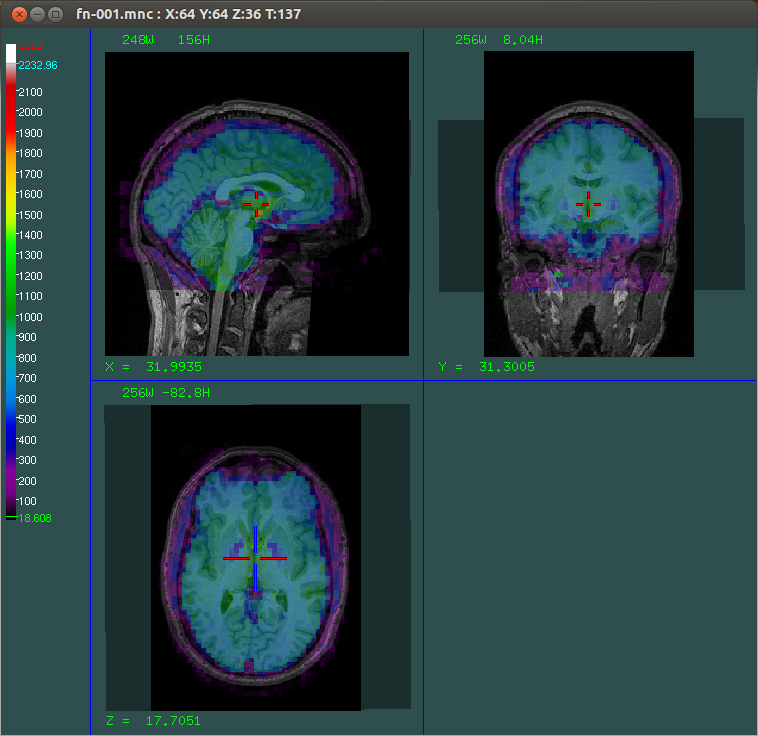
\includegraphics[width=0.6\textwidth]{display-ccode.png}
\caption{A structural and functional image overlaid in \display{}, using grayscale for the 
structural image and spectral for the functional image.}
\label{figOverlaid}
\end{figure}

Once a volume has been loaded, you can change the colour coding of the
current volume at any time by using \menu{Colour Coding} menu. You can
select one of the other colour map options, such as \menutwo{Colour
 Coding}{Spectral} or \menutwo{Colour Coding}{Gray}.

\subsection{How to Create and Save Labels}

\begin{enumerate}
\item Start \display{} the usual way, loading a volume:
\begin{verbatim}
Display prefix_104_t1_final.mnc
\end{verbatim}
\item The default paint label value is 1. To change this, click on \menutwo{Segmenting}{Set Paint Label} and then
 enter the number corresponding to the colour of the paint label that
 you want associated with painting operations. See Table \ref{tabLabCol}
for the default mapping of label values to colour names.
\item The default brush radius in the plane is 3 world units. To
 change this, click on \menutwo{Segmenting}{XY Radius} and then enter
 the desired size of the paint brush in world units.
\item You can hold down the right mouse button to draw on the current volume
using the current label value and brush size, or you can use the \menutwo{Segmenting}{Label Voxel} command to set the voxel directly under the mouse pointer.
\item If you make a mistake in drawing labels, you can undo up to the last 20
painting operations using the \menutwo{Segmenting}{Undo} command. You can also
access this command with the Ctrl-Z key combination.
\item When you wish to save the labels, you can use either the command \menutwo{File}{Save Labels .mnc} or \menutwo{File}{Save Labels .tag}. The ASCII tag file format ({\tt .tag}) may become overly large if you have defined many labels. The MINC ({\tt .mnc}) format will be more space-efficient in this case.
\item Remember that you can zoom in and out to examine more or less detail in the slice by using the scroll wheel or the shift key + middle mouse button.

\end{enumerate}

\begin{table}
\centering
\caption{Table of standard label color codes used in \display{}. Only
 the first 25 entries are shown. Entries from 14 and above are
 derived automatically from the label value and are not necessarily associated
with colour names.}
\begin{small}
\begin{tabular}{l|l|l}
Label Value & Colour Name & Colour RGB \\
\hline
1 & RED & 1.00 0.00 0.00 \\
2 & GREEN & 0.00 1.00 0.00 \\
3 & BLUE & 0.00 0.00 1.00 \\
4 & CYAN & 0.00 1.00 1.00\\
5 & MAGENTA & 1.00 0.00 1.00 \\
6 & YELLOW & 1.00 1.00 0.00 \\
7 & BLUE\_VIOLET & 0.54 0.17 0.89 \\
8 & DEEP\_PINK & 1.00 0.08 0.58 \\
9 & GREEN\_YELLOW & 0.68 1.00 0.18 \\
10 & LIGHT\_SEA\_GREEN & 0.13 0.70 0.67 \\
11 & MEDIUM\_TURQUOISE & 0.28 0.82 0.8 \\
12 & PURPLE & 0.63 0.13 0.94 \\
13 & WHITE & 1.00 1.00 1.00 \\
14 & & 0.40 0.00 0.00 \\
15 & & 0.40 0.20 0.00 \\
16 & & 0.40 0.40 0.00 \\
17 & & 0.20 0.40 0.00 \\
18 & & 0.00 0.40 0.00 \\
19 & & 0.00 0.40 0.20 \\
20 & & 0.00 0.40 0.40 \\
21 & & 0.00 0.20 0.40 \\
22 & & 0.00 0.00 0.40 \\
23 & & 0.20 0.00 0.40 \\
24 & & 0.40 0.00 0.40 \\
25 & & 0.40 0.00 0.20 \\
\hline
\end{tabular}
\end{small}
\label{tabLabCol}
\end{table}

\subsection{How to Load Labels}

You can always load labels by using the {\tt -label} option and
specifying either the {\tt .tag} or {\tt .mnc} file on the command
line:
\begin{verbatim}
Display patient_t1.mnc -label patient_t1.tag
\end{verbatim}
or 
\begin{verbatim}
Display patient_t1.mnc -label patient_t1.mnc
\end{verbatim}

If you prefer, you can load labels while \display{} is already running
by using either the \menutwo{File}{Load Labels .tag} or
\menutwo{File}{Load Labels .mnc} command as appropriate.

\subsection{How to Create a 3D Rendering of a Label}

\begin{enumerate}
\item Start \display{} the usual way, loading the volume and labels:
\begin{verbatim}
Display prefix_104_t1_final.mnc -label prefix_104_labels.mnc
\end{verbatim}
\item Click somewhere on the part of the labeled volume that you want to render as a 3D surface.
\item Go to the \menu{Create Surface} menu. 
\item Select \menutwo{Create Surface}{Label Bin-Isosurfac}.
\item Then, in the dialog window, type the MIN and MAX of the label - for example, if your value is 1, type 0.5 1.5. 
\item This performs a marching cubes rendering of the label in the objects window.
\end{enumerate}

\subsection{How to Draw a Curve on the Cortical Surface}
\begin{enumerate}
\item Start \display{}, loading a cortical surface:
\begin{verbatim}
Display prefix_104_gray_surface_left_81920.obj
\end{verbatim}
\item Select \menu{Surface Curves}.
\item Select \menutwo{Surface Curves}{Start Surf Curve} and click with left mouse button to start drawing curve on surface.
\item Click again with left mouse button on next point on surface and keep clicking to add new points to curve. Each time you click, it will connect the points using the line of shortest distance on the surface.
\item When done clicking points on surface, \menutwo{Surface Curves}{Close Curve} to finish and close the curve.
\item When done drawing curves, select \menutwo{Surface Curves}{End Surf Curve} to stop drawing surface curves entirely.
\item To save the curve, select \menutwo{Surface Curves}{Permanent Curve}, which will move the curve into the object hierarchy as a lines object.
\end{enumerate}

\subsection{How to Crop a Volume}
\begin{enumerate}
\item Start \display with your volume that you want to crop as input:  
\begin{verbatim}
Display prefix_104_t1_final.mnc
\end{verbatim}
\item Select the \menu{Volume Cropping} menu. 
\item Select the \menutwo{Volume Cropping}{Set Crop Source} and enter a file name (for example ``prefix\_104\_t1\_final.mnc'').
\item Select the \menutwo{Volume Cropping}{Pick Crop Box} command.
\item A green contour will appear around the slice planes. You can move the side of the crop window with your mouse.
\item Save the new cropped volume by pressing on \menutwo{Volume Cropping}{Crop To File} and enter a file name for the cropped volume.
\item You can now load the new cropped volume.
\end{enumerate}


\subsection{How to Display an Oblique Slice View}
\label{secOblique}
You can display an oblique (arbitrary) slice through the volume, as shown
in Figure \ref{figOblique}.
\begin{figure}
\centering
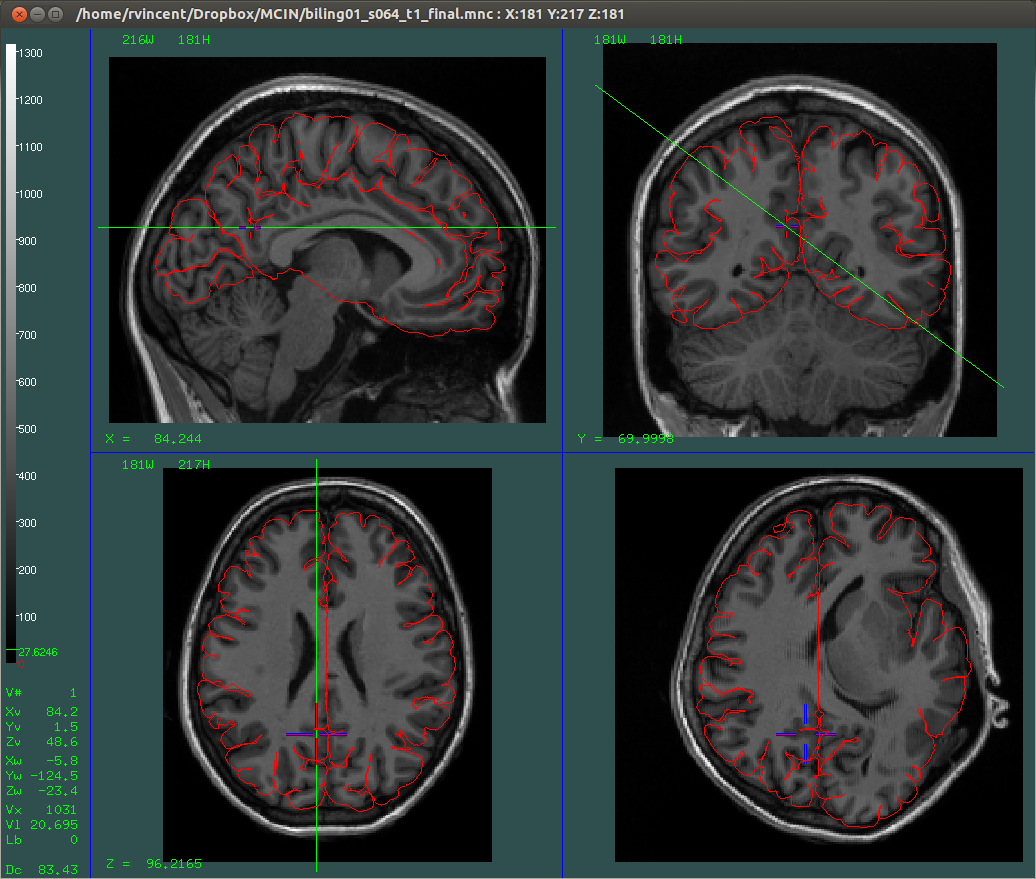
\includegraphics[width=0.6\textwidth]{display-oblique.png}
\caption{The Slice View window, demonstrating the oblique slice in the lower
right quadrant. The green lines show the intersection of the oblique slice plane with the orthogonal planes.}
\label{figOblique}
\end{figure}

\begin{enumerate}
\item Start MNI-Display as usual with a volume: 
\begin{verbatim}
Display prefix_104_t1_final.mnc 
\end{verbatim}
\item Select the \menu{Slice View} menu.
\item Move the mouse over the lower right quadrant of the slice view window.
\item Select the \menutwo{Slice View}{Toggle Slice Visibility} command to make
the fourth slice visible.
\item Select the \menutwo{Slice View}{Toggle Slice Crs-Sect} command to display slice cross section. This will display a green line which shows the intersection of the oblique plane with the current slices.
\item Select the \menutwo{Slice View}{Pick Slice Angle} command to allow you to use the left mouse button to change the angle of the oblique slice in any of the three orthogonal views.
\end{enumerate}

\subsection{How to Display Functional Activation on a Volume}

This can be done by loading both the functional volume (i.e. PET) and the anatomical cortex object.  For example, type the following:
\begin{verbatim}
Display pet_volume.mnc cortex.obj
\end{verbatim}

Then perform the following steps:
\begin{enumerate}

\item Select \menutwo{Colour Coding}{Under Colour} and set the colour to white or 0.7 0.7 0.7.
\item Select the command \menutwo{Colour Coding}{Colour Code Object}.
\end{enumerate}

Note that this procedure applies the current colour coding parameters to the current object, and after you make any change to colour coding parameters, you have to hit the \menutwo{Colour Coding}{Colour Code Object} button to cause the 3D object to be updated.

\subsection{How to Load Several Objects and Switch Between Them}

\begin{enumerate}
\item Type the following to load an average model brain and models of brainstem and cerebellum:
\begin{verbatim}
Display ti_final.mnc avg_model.obj brain_stem_model.obj cerebellum_model.obj
\end{verbatim}

\begin{figure}
\centering
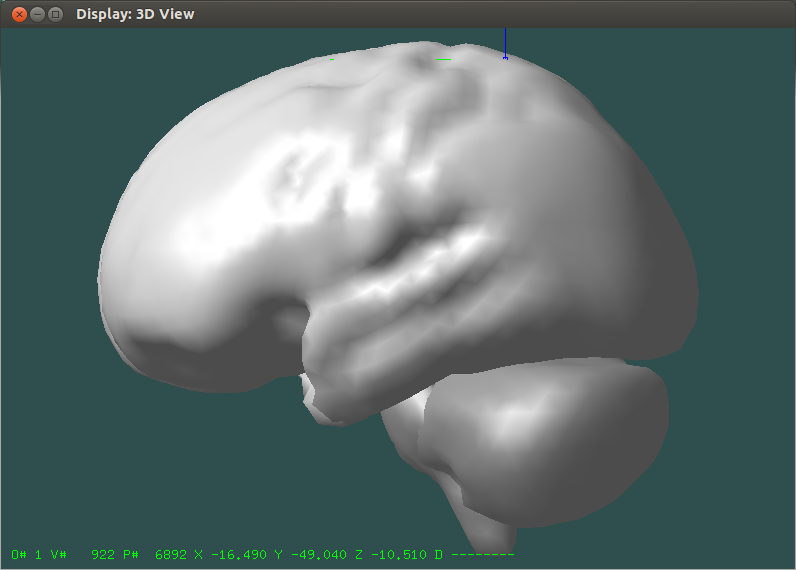
\includegraphics[width=0.5\textwidth]{display-objects.png}
\caption{The 3D View window displaying the average surface, brain stem, and
cerebellum simultaneously.}
\label{figObjects}
\end{figure}

\item Initially the 3D window displays the average model as well as the brainstem and cerebellum,  as in Figure \ref{figObjects} (use \menutwo{3D View}{Left View} to display a side view).
\item Note that the cerebellum object, the final object loaded, is the currently selected object in the Object list window.
\item Select the \menutwo{Objects}{Previous Visible} command, and the cerebellum
object will no longer be displayed. The current object will now be the brain stem object, as in Figure \ref{figNoCereb}.

\begin{figure}
\centering
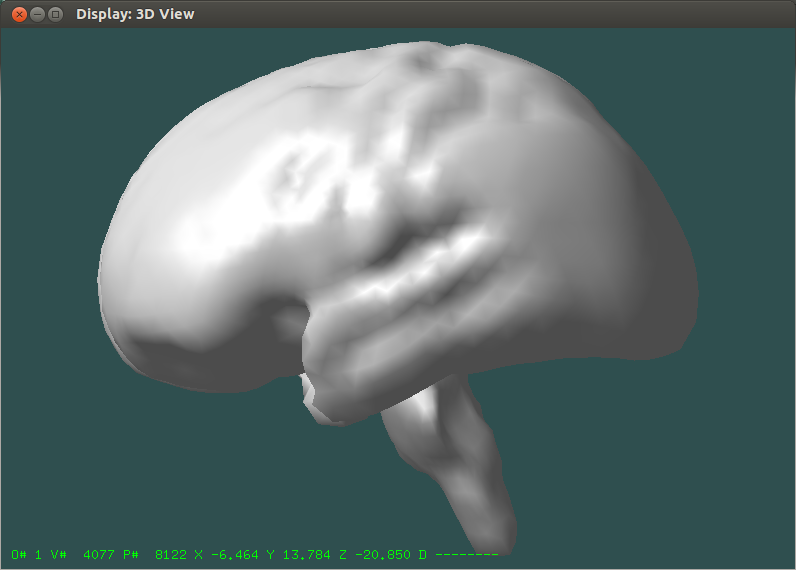
\includegraphics[width=0.5\textwidth]{display-no-cereb.png}
\caption{The 3D View window displaying the average surface, brain stem, but
not the cerebellum, which is now hidden.}
\label{figNoCereb}
\end{figure}

\item Select the command \menutwo{Objects}{Previous Visible} again, and the brain stem object will be hidden as well.
\item You can use the arrow keys and \menutwo{Objects}{Visible} or \menutwo{Objects}{Invisible} commands to select any object and change its visibility.
\item Invisible objects are not shown in either the 3D view or the slice view.
\end{enumerate}

\subsection{How to Create a Cut-Away View of a Cortical Surface}

Within MNI-Display you can create a cut-away view of the cortical surface to show anatomical features inside. Type the following to open an average model brain and model of brainstem and cerebellum:

\begin{verbatim}
Display ti_final.mnc avg_model.obj brain_stem_model.obj cerebellum_model.obj
\end{verbatim}

\begin{enumerate}
\item Rotate the 3D model, using either the \menu{3D View} menu or the middle mououse button, until you have the desired viewing angle.
\item Select the polygon object you want to crop. You may select an object either by using the arrow keys or by clicking the mouse over the object in the 3D View.
\item In the Slice View window, navigate to the slice coordinate in the view where you want to cut the object.
\item Press the key corresponding to the \menutwo{Surface Segmentation}{Crop Above} or \menutwo{Surface Segmentation}{Crop Below} command while your mouse is still over the sagittal, coronal, or transverse slice.
\item The cropped part of the polygon object will disappear.
\end{enumerate}

\subsection{How to Display a Histogram of Voxel Intensities}
The Slice View window can show a graph giving a visual indication of
the relative frequencies of different voxel values.

\begin{figure}
\centering
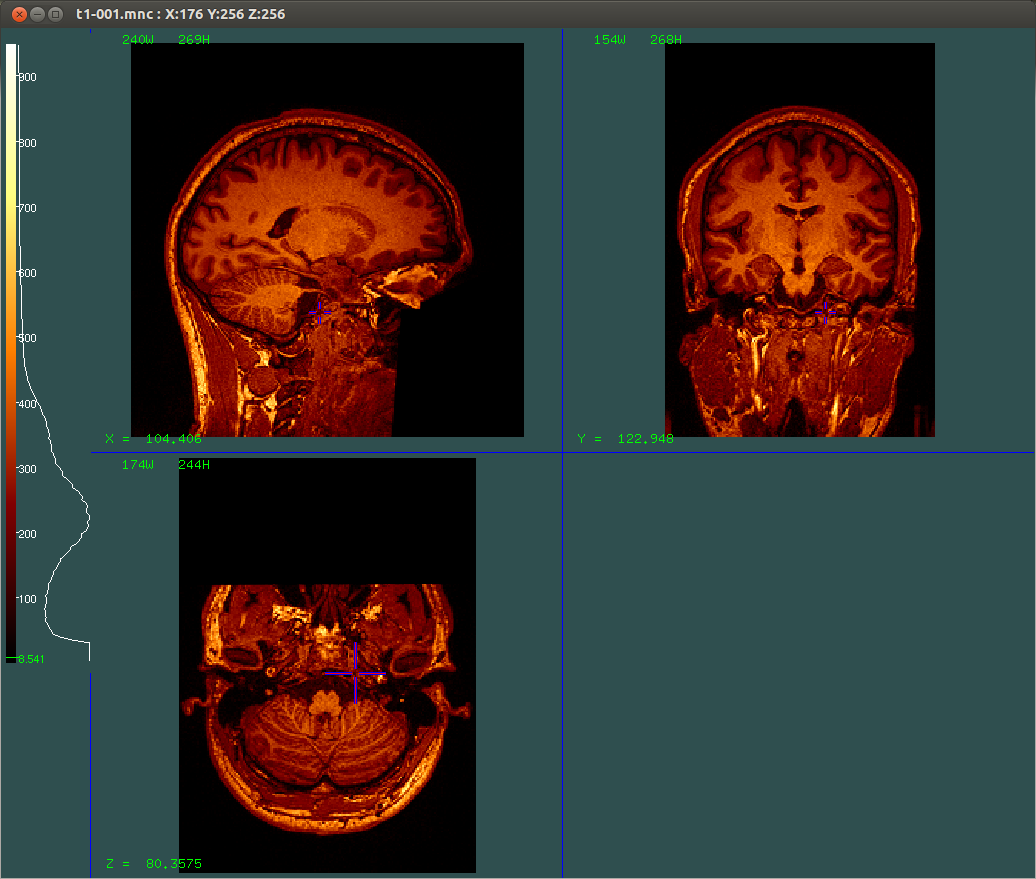
\includegraphics[width=0.6\textwidth]{display-histo.png}
\caption{The histogram appears just to the right of the colour bar in the Slice View window.}
\label{figHisto}
\end{figure}

\begin{enumerate}
\item Start \display{} as usual, opening a volume:
\begin{verbatim}
Display ti_final.mnc 
\end{verbatim}
\item Select the command \menutwo{Slice View}{Recompute Histogram}. This will
show a histogram of voxel intensities next to the colour bar scale.
\item If the mouse is over a particular slice when the command is selected, the histogram will reflect the intensities of that slice only. Otherwise, the histogram will be taken over the entire volume.
\item You have to explicitly choose the \menutwo{Slice View}{Recompute Histogram} command to update the histogram.
\end{enumerate}

\subsection{How to Create a Cortical Surface from a Volume}
\begin{enumerate}
\item Start \display{} as usual, opening a volume:
\begin{verbatim}
Display prefix_104_ti_final.mnc 
\end{verbatim}
\item Switch to \menutwo{Colour Coding}{Gray Scale}.
\item Select the \menu{Create Surface} menu.
\item Move mouse on volume to position where surface extraction should start.
\item Select the \menutwo{Create Surface}{Volume Isosurface} command
\item Type isovalue into Text Input window (e.g. 140).
\item The surface will be extracted and will appear in 3D window. This operation
can take some time.
\item If the surface extraction does not work properly, you can select \menutwo{Create Surface}{Reset Surface} to remove the existing surface and try again with a different isovalue or a different starting location in the Slice window.
\item The extracted surface can then be smoothed using \menutwo{Polygons}{Smooth Polygon}.
\end{enumerate}

\section{What is the Object (.obj) File Format}

The .obj format is a simple format to store polygons, lines, and other
geometric objects. The format supports both ASCII text and binary versions, you can choose which format \display{} uses by setting the Save\_format global in your configuration file. In general, the ASCII format is preferred as it is more likely to be portable among different machines.

The format is described in detail elsewhere, as part of the
documentation of the BICPL library. You can access the \LaTeX{}
sources of the document at this URL:
\url{https://github.com/BIC-MNI/bicpl/blob/master/Documentation/mni_obj_format.tex}

%% Commented out until we actually have something to say that is true 
%% and useful.
%% \section{Running \display{} on Mac OS X}

%% \subsection{How to Display 3D Window on Mac}

%% \subsection{How to Set Preferences on Mac}

%% \subsection{Object Hierarchy on the Mac}

\section{Configuration variables}
\label{secGlobals}

\display{} includes many ``global variables'' that can be set in a
configuration file, from the command line, or using a command within
the program.  These globals serve a wide range of
purposes - they may control the appearance of the user interface, set
parameters for surface extraction, control editing behavior, or even
affect low-level graphics performance. Many of the globals are not
intended to be changed during program execution, as their values may
only be read at startup. Others can be changed dynamically while the
program is running, and may take effect immediately. Some globals are
set implicitly by specific commands in the \display{} user interface.

Most of these globals have not been rigorously tested over their
entire possible range. Input checking is often minimal. It is
therefore possible to alter the behavior of the program in unexpected
or confusing ways. This document will not be comprehensive, but will
attempt to explain some of the most useful variables.

Every global variable has a name and a type, and the program will only
accept values it recognizes as being in the proper type. 

Variable names typically start with an initial capital letter and
consist of several descriptive words separated by underscores. In all
contexts, \display{} requires that the name be given exactly as
specified, with the correct capitalization.

Variable types may be one of the following:
\begin{itemize}
\item String - Any string of ASCII characters.
\item Boolean - A string representing a boolean (true or false) value. Only the first character of the string is examined, with a 't' or `T' indicating true and an 'f' or 'F' indicating false.
\item Integer - A whole decimal number.
\item Real - A decimal number with an optional fractional part.
\item Point - A set of three floating-point number
s specifying a position
along the X,Y, and Z axes.
\item Vector - A set of three floating-point numbers specifying a direction
along the X,Y, and Z axes.
\item Colour - Either a string that gives a colour name (e.g. ``BLUE'') or a series of 3 or 4 numbers specifying RGB or RGBA values in the range 0-1.
\item Surface property - A set of five floating-point parameters that give
the surface properties of an object.
\end{itemize}

Certain types, especially String or Integer, may have other
interpretations depending on the specific variable. For example, some
strings may be interpreted as filenames or formatting strings.

\subsection{Setting globals in a configuration file}
The most reliable way to set global variables is through the configuration file, which is loaded very early in the initialization process. Many of the configuration values are used only during program initialization, so setting them from the command line or the internal command may have no effect!

By default, the configuration file is named {\tt Display.globals}, and
it is most commonly located in the user's home directory. However, the 
program searches for the file in each of the following locations, in order:
\begin{enumerate}
\item /usr/local/lib/
\item The hard-coded installation directory for the package.
\item The directory that contains the binary image for \display.
\item The user's home directory.
\item The current directory ('.').
\end{enumerate}

Note that if a file named {\tt Display.globals} is present in any of these
directories, each such file will be loaded. Therefore it is possible
for later configuration files to add or replace values set in
previously loaded configuration files.

We have recently added a separate configuration file named {\tt
 .mni-displayrc} which is identical in syntax to {\tt
 Display.globals}, but which is intended only for internal use by the
program. It may be overwritten by certain commands in the user interface.

A configuration file consists of a series of lines consisting of a
variable name, followed by one or more spaces, an equals sign ('='),
and finally a variable value. Each line is terminated with a semicolon
(';'). Comments may be included by using a hash ('\#') as the first character
on a line. Comments and empty lines are ignored.

Here is an example {\tt Display.globals} file:
\begin{verbatim}
# Here is a comment.
Default_marker_label = Hippocampus;
#Default_marker_size = 0.02;
Hide_3D_window = false;
Hide_marker_window = false;
Atlas_filename = /data1/users/bert/talairach/Talairach_atlas.list
Max_polygon_scan_distance=0.5;
Object_outline_enabled = True;
Convert_volumes_to_byte=False;
Slice_readout_text_font = 0;
Display_frame_info = True;
\end{verbatim}


\subsection{Setting globals on the command line}

A global can be set from the command line by specifying the {\tt
 -global} command line option. The command line is parsed after the
configuration files are loaded, so values specified on the command
line may override the setting in the configuration files. This will
not be true for all globals, as many of them are only used during the
earliest part of program initialization.

The command line option takes a variable name and value separated from
the option by spaces:
\begin{verbatim}
Display -global Default_paint_label 5 my_t1_image.mnc
\end{verbatim}
This example will set the initial value used for voxel labeling (``painting'') to 5 instead of the default, which is 1.

You can repeat the {\tt -global} option as many times as you like, to
set any number of globals.

\subsection{Setting globals with a menu command}

The \menutwo{Quit}{Global Var} menu command allows you to inspect or
change the value of any global variable. In the default menu structure,
this command is accessed from the ``Quit'' sub-menu, so one can invoke
the command by pressing the '7' key followed by the 'A' key. This will
prompt you to enter a string. If you simply want to check the value of a
variable, you may just enter the variable's name and press Enter. If you
want to change the variable's value, you enter the variable's name
followed by an equals sign ('=') and the desired new value.

Again, be warned that, as with the command line, changing some globals
through this menu command will have no effect. Not all globals will take 
effect after \display{} has been initialized.

\subsection{List of useful globals}

\newcommand{\globalentry}[5]{\subsubsection{{\tt #1}}
\paragraph{Type}{#2}%
\paragraph{Default value}{#3}%
\paragraph{Description}{#4}%
\if\relax\detokenize{#5}\relax%
  %
  \else
  \paragraph{Command}{#5}%
  \fi
}

\globalentry{Atlas\_filename}
{String}{/avgbrain/atlas/talairach/obj/Talairach\_atlas.list}
{Gives the location for the list of Talairach atlas files.}{}

\globalentry{Closest\_front\_plane}
{Real}{1.0e-5}
{Sets the smallest position of the front plane used in 3D rendering.}{}

\globalentry{Convert\_volumes\_to\_byte}
{Boolean}{False}
{If true, volumes are converted to byte as they are loaded, which reduces the possible number of intensities to 256. Set this to false if you need to visualize a file with a higher precision.}{}

\globalentry{Colour\_below}
{Colour}{Black}
{The colour to display for all voxels that lie below the current minimum
 value of the colour coding range.}{}

\globalentry{Colour\_above}
{Colour}{White}
{The colour to display for all voxels that lie above the current maximum
 value of the colour coding range.}{}

\globalentry{Crop\_label\_volume\_threshold}
{Real}{0.9}
{Sets the maximum size ratio for label volume cropping. If cropping is enabled,
 output label volumes will only be cropped if the size of the resulting
 volume is less than this value times the original size.}{}

\globalentry{Cursor\_home}
{Point}{0 0 0}
{Sets the ``home'' location of the cursor in world coordinates, used by 
\menutwo{Markers}{Move Cursor Home}.}{}

\globalentry{Cursor\_rgb\_colour}
{Colour}{Blue}
{Defines the colour of the small box at the centre of the cursor in the 3D window. The colours of the three axes lines are fixed at X=RED, Y=GREEN, Z=BLUE.}{}

\globalentry{Default\_paint\_label}
{Integer}{1}
{The initial value used to label voxels when painting the slice window.}
{{\bf F} Segmenting / {\bf D} Set Paint Lbl}

\globalentry{Default\_x\_brush\_radius}{Real}{3.0}{Default width of the
 primary brush in world units.}{}

\globalentry{Default\_y\_brush\_radius}{Real}{3.0}{Default height of the
primary brush in world units.}{}

\globalentry{Default\_z\_brush\_radius}{Real}{0.0}{Default depth of the
 primary brush in world units.}{}

\globalentry{Draw\_brush\_outline}
{Boolean}{True}
{If true, the outline of the current brush shape will be drawn as voxels are painted in the slice window. If false, only the altered voxel labels themselves will be drawn.}{}

\globalentry{Hide\_3D\_window}
{Boolean}{True}
{If true, the 3D window will be hidden by default. However, if any surface or other geometric objects are loaded, this option will be overridden and the 3D window will be displayed in any case.}{}

\globalentry{Hide\_marker\_window}{Boolean}{True}
{If true, the object list window will be hidden by default. However, if any surface or other geometric objects are loaded, this option will be overridden and the object list window will be displayed in any case.}{}

\globalentry{Hide\_menu\_window}
{Boolean}{False}
{If true, the menu window will be hidden. Command keystrokes will continue to work normally, but the virtual keyboard will not be available.}{}

\globalentry{Histogram\_colour}
{Colour}{WHITE}
{Sets the colour of the histogram curve, as drawn in the slice window if requested.}{}

\globalentry{Initial\_background\_colour}
{Colour}{0.184314, 0.309804, 0.309804} 
{Sets the background colour of each of the windows. Only
the slice window is created late enough for this to have an effect
from the command line, and it has no effect if changed from the menu
command. For some inexplicable reason, the default dark greenish
background is given the symbolic name {\tt DARK\_SLATE\_GREY}. While the
background colour can be changed through a menu command, the command will not
change the colour for the menu or object windows.}{}

\globalentry{Initial\_coding\_range\_absolute}{Boolean}{False}{If true,
the variables Initial\_coding\_range\_low and
Initial\_coding\_range\_high are interpreted as absolute upper and lower
bounds on the initial colour coding range. If false, they are treated as 
fractions of the actual range.}{}

\globalentry{Initial\_coding\_range\_high}{Real}{0.75}{If
  Initial\_coding\_range\_absolute is true, this variable sets the
  initial value of the high range of the colour coding. If
  Initial\_coding\_range\_absolute is false, this value is interpreted
  as a fraction of the actual range.}{}

\globalentry{Initial\_coding\_range\_low}{Real}{0.25}{If
  Initial\_coding\_range\_absolute is true, this variable sets the
  initial value of the low range of the colour coding. If
  Initial\_coding\_range\_absolute is false, this value is interpreted
  as a fraction of the actual range.}{}

\globalentry{Initial\_colour\_coding\_type} {Integer}{1} {Sets the
  colour coding scheme used by the first loaded volume in the slice
  window. The most useful values are 0 for grayscale, 1 for hotmetal,
  13 for spectral, 14 for red, 15 for green, 16 for blue, and 17 for
  contour. Other possibly useful values include 3 for ``cold metal'',
  5 for ``green metal'', 7 for ``lime metal'', 9 for ``red metal'',
  and 11 for ``purple metal''.}{}

\globalentry{Initial\_histogram\_contrast}
{Boolean}{True}
{If true, \display{} will calculate a histogram of each loaded volume
  and use it to set the initial colour coding range. The low range will
  be set attempt to keep Initial\_histogram\_low voxels below the range,
  and Initial\_histogram\_high voxels above the range.}{}

\globalentry{Initial\_histogram\_high}
{Real}{0.99999}
{If this Initial\_histogram\_contrast flag is true, this variable
  determines the percentile used for the initial high colour range.}{}

\globalentry{Initial\_histogram\_low}
{Real}{0.2}
{If this Initial\_histogram\_contrast flag is true, this variable
  determines the percentile used for the initial low colour range.}{}

\globalentry{Initial\_histogram\_low\_clip\_index}
{Integer}{4}
{If this Initial\_histogram\_contrast flag is true, this variable
 determines the number of bins to ignore from the low portion of the 
histogram. In other words, by default we don't consider histogram bins
0-3 to contribute to the percentiles used to calculate the range.}{}

\globalentry{Initial\_label\_colour\_table} {Integer}{0}
{This variable controls the normal or default colours used for labels
in \display{}. A value of zero (the default) selects the 'classic'
colour table used in \display{} for many years. However, this table
has known deficiencies, including many repeated colours. A value of
1 selects a standard colour table that is used in other tools at
the MNI. A value of 2 selects an experimental colour table that
attempts to maximize the visual distance between colours.}{}

\globalentry{Initial\_perspective\_flag}
{Boolean}{False}
{Sets the initial value of the projection approach used in 3D rendering. A value of false selects parallel projection, whereas true selects perspective projection.}
{{\bf W} 3D view / {\bf D} Proj}

\globalentry{Initial\_render\_mode}
{Boolean}{True}
{If true, 3D objects are rendered in shaded mode by default. If false, 3D objects are rendered in wireframe mode by default.}
{{\bf E} 3D Render / {\bf A} Mode}

\globalentry{Initial\_shading\_type}
{Integer}{1}
{Selects either Gouraud (1) or flat (0) shading as the default used in the 3D window.}
{{\bf E} 3D Render / {\bf S} Shading}

\globalentry{Initial\_slice\_continuity}{Integer}{-1} 
{Selects either nearest-neighbour (-1), trilinear (0), or tricubic (2) for the
 initial slice interpolation method.}{}

\globalentry{Initial\_undo\_feature}
{Boolean}{True}
{Determines the initial state of the ``undo'' option. Set to false if you want undo disabled by default, but wish to leave it under user control. To disable undo completely, set Undo\_enabled to false.}
{{\bf F} Segmenting / {\bf M} Enable Undo}

\globalentry{Menu\_character\_colour} {Colour}{CYAN}
{For active commands, sets the colour of the command name text
  associated with each virtual key in the menu window.}{}

\globalentry{Menu\_character\_inactive\_colour} {Colour}{SLATE\_GREY}
{For inactive commands, sets the colour of the command name text
  associated with each virtual key in the menu window.}{}

\globalentry{Menu\_box\_colour}
{Colour}{WHITE}
{Sets the colour of the box that outlines each virtual key in the menu window.}{}

\globalentry{Menu\_key\_colour}
{Colour}{WHITE}
{Sets the colour of the key name associated with each virtual key in the menu window.}{}

\globalentry{Move\_slice\_speed}
{Real}{0.25}
{Sets the speed at which the slice is changed when the middle button is pressed in the slice window. Use a smaller number to make the slice change more slowly.}{}

\globalentry{Object\_outline\_enabled}
{Boolean}{True}
{If true, any graphics object or surface that is visible in the 3D window will also be displayed by projecting its outline onto the planes of the slice window.}{}

\globalentry{Object\_outline\_width}
{Real}{1.0}
{Sets the line width used when drawing the projection of 3D objects on the planes of the slice window.}{}

\globalentry{Pixels\_per\_double\_size}
{Real}{100.0}
{Sets the number of pixels the cursor must move to double the zoom level when using the original ``shift+middle button'' zoom in the slice window. Smaller numbers yield give faster zooming.}{}

\globalentry{Save\_format} {Integer}{0} {Controls whether graphical
 objects will be saved in ASCII (0) or binary (1) format. In general,
 ASCII format is more likely to be portable among different machine
 architectures.}{}

\globalentry{Scalebar\_colour}{Colour}{CYAN}{
The colour to use for the scalebar.
}{}

\globalentry{Scalebar\_enabled}{Boolean}{False}{
If TRUE, scalebar display on the slice view is enabled.
}{}

\globalentry{Scalebar\_height}{Integer}{8}{
Height of the scalebar in pixels.
}{}

\globalentry{Scalebar\_quadrant}{Integer}{1}{
Set the quadrant of the scalebar, one of the following:
1: upper right, 2: upper left, 3: lower left, 4: lower right
}{}


\globalentry{Secondary\_x\_brush\_radius}{Real}{3.0}{Defines the width
 of the secondary brush in world units.}{}

\globalentry{Secondary\_y\_brush\_radius}{Real}{3.0}{Defines the height
 of the secondary brush in world units.}{}

\globalentry{Secondary\_z\_brush\_radius}{Real}{3.0}{Defines the depth
  of the secondary brush in world units.}{}

\globalentry{Show\_cursor\_contours}
{Boolean}{False}
{If true, the ``cursor contours'' will be displayed in the 3D
  view. These contours are defined by the intersection between the slice
  view planes and the 3D objects.}{}

\globalentry{Show\_markers\_on\_slice}
{Boolean}{True}
{True if Display should draw the outlines of markers in the slice window.}
{}

\globalentry{Show\_slice\_field\_of\_view}
{Boolean}{False}
{If true, displays the current width and height of the field of view of
  each panel in the slice window.}{}

\globalentry{Single\_window}
{Boolean}{False} 
{If true, \display{} will combine all four different user interface
 windows into a single large window. This is still an experimental
 feature, provided for purposes of eliciting user feedback. This
 variable must be set in {\tt Display.globals} for it to take effect.}{}

\globalentry{Slice\_change\_fast}
{Integer}{10}
{Sets the amount by which to multiply {\tt Slice\_change\_step} when
  changing slice using the '[' or ']' keys.}{}

\globalentry{Slice\_change\_step}
{Integer}{1}
{Sets the number of slices to move when the '+' or '-' keys are
  pressed.}{}

\globalentry{Slice\_cross\_section\_colour}
{Colour}{GREEN}
{Sets the colour of the slice cross section, the projection of the oblique cross section plane in the three orthogonal planes in the slice window.}{}

\globalentry{Slice\_cursor\_colour1}
{Colour}{RED}
{Sets the color of the ``inner'' part of the slice windows's cursor.}{}

\globalentry{Slice\_cursor\_colour2}
{Colour}{BLUE}
{Sets the color of the ``outer'' part of the slice windows's cursor.}{}

\globalentry{Slice\_divider\_colour}
{Colour}{BLUE}
{Sets the colour of the slice dividers, the lines that define the four quadrants of the slice window.}{}

\globalentry{Slice\_divider\_x\_position}
{Real}{0.5}
{Sets the initial X position of the slice dividers, as a fraction of the overall slice view area.}{}

\globalentry{Slice\_divider\_y\_position}
{Real}{0.5}
{Sets the initial Y position of the slice dividers, as a fraction of the overall slice view area.}{}

\globalentry{Slice\_readout\_text\_font}
{Integer}{0}
{Selects either a fixed-width (0) or proportional-spaced (1) font for the
coordinate and value information displayed in the lower-left corner of the slice window.}{}

\globalentry{Tags\_from\_label}
{Boolean}{False}
{If true, \display{} will attempt to automatically maintain a list of
 tags associated with each label. A marker object will be created
 corresponding an example location that has been marked with each label
 value. A marker will be removed if all of the voxels associated
 with its label value are erased.
 This is still quite experimental and may produce unexpected results.}{}

\globalentry{Undo\_enabled}
{Boolean}{True}
{Determines whether or not the ``undo'' option is {\em ever} enabled when painting the slice window. The undo function requires memory and processing time that may be impractical with very high resolution images. This option silently disabled the undo feature without giving the user the opportunity to turn in back on in the menu.}{}

\globalentry{Use\_cursor\_origin}
{Boolean}{True}
{If true, certain operations, such as rotation of the 3D image, are centered on the current cursor origin. If false, the rotations are centered on the middle of the window.}{}

\globalentry{Use\_zenity\_for\_input}
{Boolean}{True}
{If true, \display{} will attempt to use the Zenity program for user interaction
such as prompts for file names and other user input. If false, 
\display{} will revert to using the terminal window for all user interaction.}{}

\globalentry{Visibility\_on\_input}
{Boolean}{True}
{If true, \display{} will make newly-loaded 3D objects visibile immediately.}{}

\subsection{List of developer globals}
These globals are useful primarily for developers or when debugging problems
with \display. They may be removed or changed with little notice.

\globalentry{Alloc\_checking\_enabled}
{Boolean}{False}
{Enables memory allocation checks. This is primarily intended for use by developers when debugging problems in \display.}{}

\globalentry{Display\_frame\_info}
{Boolean}{False}
{If true, adds an indication of the frame number and elapsed rendering time to the lower left corner of each of the graphics windows. The actual position is determined by the globals {\tt Frame\_info\_x} and {\tt Frame\_info\_y}}{}

\globalentry{Min\_interval\_between\_updates}{Real}{0.02}
{Sets the number of seconds between timer events. Each timer event may
start another redraw operation, so this variable controls the maximum
frame rate of the application.}{}



\end{document}
